
\section{Coins}

%\section{Summary}
%\seclabel{Summary}
{\it In this introductory chapter we lay the conceptual foundation for the rest 
of what we have to say about redeveloping economic theory. We play a simple coin-toss game and analyze it 
numerically, by Monte Carlo simulation, and analytically, with pen and paper. The game motivates the 
introduction of the expectation value and the time average, which in turn 
lead to a discussion of ergodic properties. Ergodicity will turn out to be the key concept that was not understood -- because it hadn't been discovered -- in the initial development of formal economics. We note the importance of rates 
of change and introduce Brownian motion and Geometric Brownian motion.
Some historical perspective is provided to understand the prevalence or
absence of key concepts in modern economic theory and other fields.
The emphasis is on concepts, with more formal treatments and applications
in later chapters.}
\newpage

\subsection{The game}
\seclabel{The_game}
Imagine we offer you the following game: we toss a coin, and if it comes 
up heads we increase your monetary wealth by 50\%; if 
it comes up tails we reduce your wealth by 40\%. We're not only 
doing this once, we will do it many times, for example 
once per week for the rest of your life. Would you accept 
the rules of our game? Would you submit your wealth to 
the dynamic our game will impose on it?

Your answer to this question is up to you and will be 
influenced by many factors, such as the importance 
you attach to wealth that can be measured in monetary 
terms, whether you like the thrill of gambling, your 
religion and moral convictions and so on.

In these notes we will mostly ignore these factors.
We will build an extremely simple model of your 
wealth, which will lead to an extremely simple and 
powerful model of the way you make decisions that affect 
your wealth. We are interested in analyzing the 
game mathematically, which requires a translation 
of the game into mathematics. We choose the 
following translation: we introduce the key 
variable, $\x(\t)$, which we refer to as ``wealth''. 
We refer to $\t$ as ``time''. It should be kept in mind that
``wealth'' and ``time'' are just names that we've given to 
mathematical objects. We have chosen these names because
we want to compare the behaviour of the mathematical
objects to the behaviour of wealth over time, but
we emphasize that we're building a model -- whether we write $\x(\t)$, 
or $\text{wealth}(\text{time})$, or \smiley(\lightning) makes no difference to the mathematics. 

The usefulness of our model will be different in different circumstances, 
ranging from completely meaningless to very helpful. There is no 
substitute for careful consideration of any given situation, and
labeling mathematical objects in one way or another is certainly none.

Having got these words of warning out of the way, we define our 
model\footnote{For those in the know: ``our'' coin toss is a discrete version of geometric Brownian motion, the workhorse model of financial mathematics and much more.} of the dynamics of your wealth under the rules we just specified. 
At regular intervals of duration $\dt$ we randomly generate a 
factor $\gr(\t)$ with each possible value
$\gr_i\in \{0.6, 1.5\}$ occurring with probability 1/2, 

\be 
\gr(\t) = \begin{cases}
0.6 &\text{with probability  1/2}\\
1.5 &\text{with probability 1/2}
\end{cases}
\elabel{law}
\ee
and multiply current wealth by that factor, so that
\be
\x(\t)=\gr(\t)\x(\t-\d \t).
\elabel{gamble}
\ee

We have good reasons to suspect that this model will do something interesting. It's not just a silly game because it has one important property: it's multiplicative. Every time the coin is tossed, wealth is {\it multiplied} by one of the two possible factors. This introduces a reference point, or state-dependence, of the absolute size of the change. Processes with this property are very common in nature -- the amount of anything that reproduces changes in proportion to what's already there. In the absence of other constraints, such as limited resources, this applies to the dynamics of the biomass of a cell culture. In fact, life itself has been defined as that which produces more of itself \cite{Morowitz1992}: life and evolution begin with the minimal chemical structure that can copy itself. The rest, in a sense, is details. We will see, especially in \cref{Interactions}, how multiplicativity generates interesting structure in -- including but not limited to -- economics.

Without discussing in depth how realistic a representation of your 
wealth this model is (for instance your non-gambling related 
income and spending are not represented in the model),
 and without discussing whether randomness truly exists and 
what the meaning of a probability is we simply switch on a 
computer and simulate what might happen. You may have many 
good ideas of how to analyze our game with pen and paper, 
but we will just generate possible trajectories of your wealth 
and pretend we know nothing about mathematics or 
economic theory. \Fref{1_1} is a trajectory of your wealth, 
according to our computer model as it might evolve over 
the course of 52 time steps (corresponding to one year given our 
original setup).

\begin{figure}[h!]
\begin{picture}(200,190)(0,0)
    \put(0,0){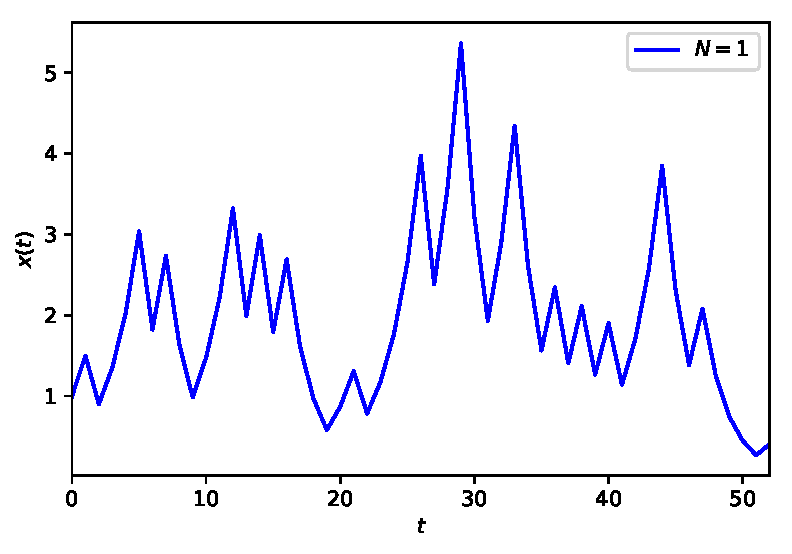
\includegraphics[width=\textwidth]{./chapter_coins/figs/x_of_t_lin_1.pdf}}
\end{picture}
\caption{Wealth $\x(\t)$ resulting from a computer simulation of our game, as specified by \eref{law} and \eref{gamble}, for 52 time steps (corresponding to one year in the given setup).}
\flabel{1_1}
\end{figure}


A cursory glance at the trajectory does not reveal much structure. 
Of course there are regularities, for instance at each time step 
$\x(\t)$ changes, but no trend is discernible -- does this trajectory 
have a tendency to go up, does it have a tendency to go down? 
Neither? What are we to learn from this simulation? Perhaps we 
conclude that playing the game for a year is quite risky, but is the 
risk worth taking? 

\subsubsection{Averaging over many trials}
The trajectory in \fref{1_1} doesn't tell us much about overall tendencies.
There is too much noise to discern a clear signal. A common 
strategy for getting rid of noise is to try again. And then try again and
again, and look at what happens on average. 
An example of the technique is Shannon's error-correcting code:
instead of sending the message $0$ (or $1$), send the relevant digit 3 times. The recipient averages over the received digits and takes the closest possibility. If one out of three digits was miscommunicated because of noise, the code nonetheless recovers the original message: averaging gets rid of noise.
%For example, this is 
%very successful in imaging -- the 2014 Nobel Prize in chemistry 
%was awarded for a technique that takes a noisy image again and 
%again. By averaging over many images the noise is reduced and 
%\href{https://en.wikipedia.org/wiki/Super-resolution_microscopy#Stochastic_functional_techniques}{a resolution beyond the diffraction limit is achieved}.

So let's try this in our case and see if we can make sense of the game.
In \fref{1_2} we average over a finite number, $N$, of
trajectories. We call a collection of trajectories an ensemble. We shall see that in the limit $N\to\infty$ the ensemble average converges to the expectation value, and indeed the terms ``ensemble average'' and ``expectation value'' are synonyms. To avoid confusion we will be explicit when $N$ is finite: in \fref{1_2} we plot ``finite-ensemble averages.''

\begin{defn}{Finite-ensemble average} The finite-ensemble average of the quantity 
$z$ at a given time $\t$ is
\be
\ave{\z(\t)}_{\N}=\frac{1}{\N}\sum_{\gi}^{\N} \z_{\gi}(\t),
\elabel{f_ens}
\ee 
where $\gi$ indexes a particular realization of $\z(\t)$ and $\N$ is the
number of realizations included in the average.
\end{defn}
\begin{figure}[h!]
\begin{picture}(200,200)(0,0)
    \put(-100,0){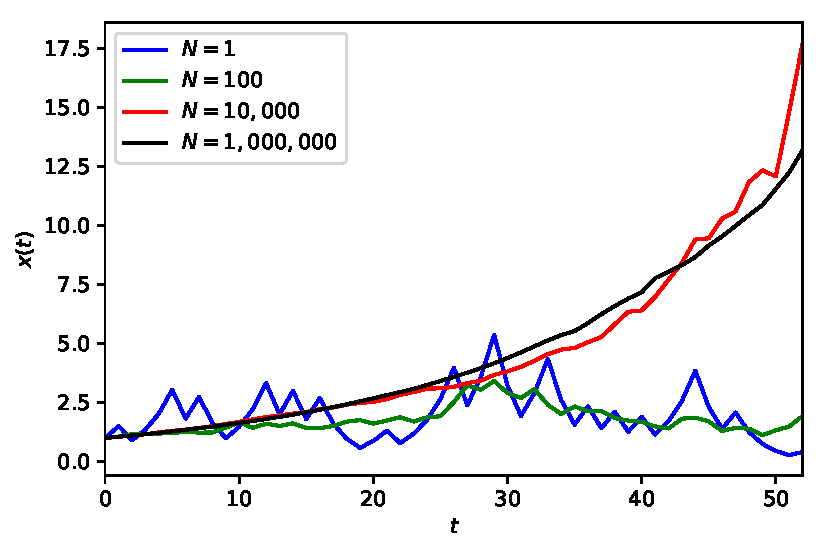
\includegraphics[width=0.8\textwidth]{./chapter_coins/figs/x_of_t_lin.pdf}}
  \put(-50,30){(A)}
  \put(180,0){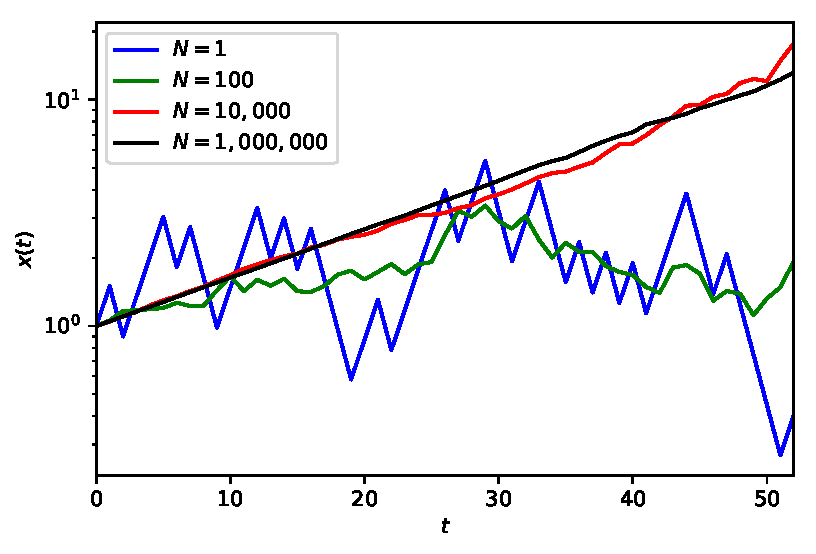
\includegraphics[width=0.8\textwidth]{./chapter_coins/figs/x_of_t_log.pdf}}
  \put(230,30){(B)}  
\end{picture}
\caption{Finite-ensemble averages $\ave{\x(\t)}_{\N}$ for ensemble sizes $\N=1, 
10^2, 
10^4, 10^6$. The noise in the finite-ensemble average diminishes systematically as $\N$ increases. 
(A) on linear scales the multiplicative (non-linear) nature of the process is apparent, (B) on logarithmic scales the multiplicative process is additive in time, and the finite-ensemble average for $\N=10^6$ is a straight line except for small fluctuations.}
\flabel{1_2}
\end{figure}
\FloatBarrier
As expected, the more 
trajectories are included in the average, the smaller the fluctuations of 
that average. For $\N=10^6$ hardly any fluctuations are visible. Since the 
noise-free trajectory points up it is tempting to conclude that my own wealth will similarly go up and  conclude that the risk 
of the game is worth taking. This reasoning has dominated economic 
theory for about 350 years now. But it is flawed. The correction of this flaw and its far-reaching consequences constitute our research program.

\subsubsection{Averaging over time}
Does our analysis necessitate the conclusion that the gamble is worth taking? 
Of course it doesn't, otherwise we wouldn't be belabouring this point. 
 Our critique will focus on the type of averaging we have applied -- we didn't play the game many times
in a row as would correspond to the real-world situation of repeating the game once a week for the rest of your life. 
Instead we played the game many times in parallel, which corresponds to a different setup\footnote{This different setup would correspond splitting our wealth into $\N$ equal parts and bet each in a sequence of independent coin tosses. But the rules of our game as we defined it don't allow that.}.

We therefore try a different analysis. \Fref{1_3} shows another simulation of your wealth. This time we don't show an average over many trajectories but a simulation of a single trajectory
over a long time. Noise is removed also in this case but in a different way: to capture visually what 
happens over a long time we have to zoom out -- more time has to be represented by 
the same amount of space on the page. In the process of this zooming-out, small 
short-time fluctuations will be diminished. Eventually the noise will be removed from the system 
just by the passage of time.

\begin{figure}[h!]
\begin{picture}(200,200)(0,0)
    \put(-100,0){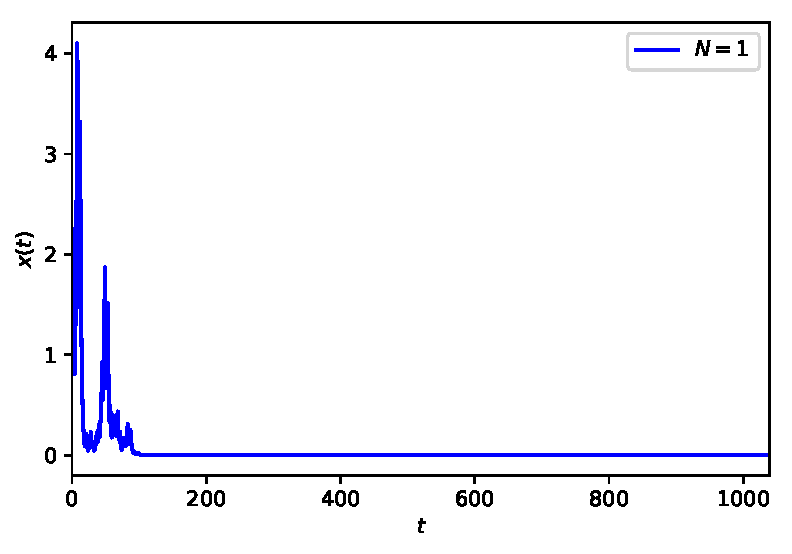
\includegraphics[width=0.75\textwidth]{./chapter_coins/figs/x_of_t_lin_20_year.pdf}}
  \put(-50,30){(A)}
  \put(180,0){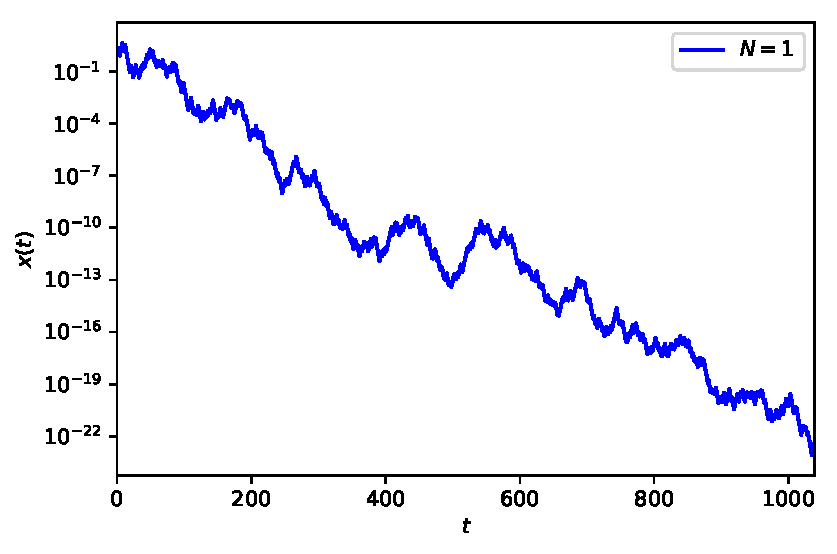
\includegraphics[width=0.8\textwidth]{./chapter_coins/figs/x_of_t_log_20_year.pdf}}
  \put(230,30){(B)}  
\end{picture}
\caption{Single trajectory over 1,040 time steps, corresponding to 20 years 
in our 
setup. (A) on linear scales all we see is wealth quickly dropping to zero, (B) logarithmic scales are more appropriate for the multiplicative process and reveal systematic exponential decay.}
\flabel{1_3}
\end{figure}
\FloatBarrier

The trajectory in \fref{1_3} is, of course, random, but the apparent trend emerging from the randomness 
strongly suggests that our initial analysis in \fref{1_2} does not reflect what happens over time in a single system. 
%Jumping ahead a little, we reveal that this is indeed the case. If it seems counter-intuitive then this is 
%because our intuition is built on so-called ``ergodic processes'', whereas $\x$ is non-ergodic. We will say
%more about this in \secref{Ergodic_observables}.
Several important messages can be derived from the observation that an individual trajectory grows 
more slowly (or decays faster) over time than an average of a large ensemble. 

\begin{enumerate}
\item
An individual whose wealth follows \eref{gamble} will make poor decisions if he uses the 
finite-ensemble average of wealth as an indication of what is likely to happen to his own wealth.
\item
The performance of the average (or aggregate) wealth of a large group of individuals differs systematically from 
the performance of an individual's wealth. In our case large-group wealth grows (think \GDP), whereas 
individual wealth decays.
\item
For point 2 to be possible, \ie for the average to outperform the typical individual, wealth must 
become increasingly concentrated in a 
few extremely rich individuals. The wealth of the richest individuals must be so large that the average becomes 
dominated by it, so that the average can grow although almost everyone's wealth decays. Inequality 
increases in our system.
\end{enumerate}

The two methods we've used to eliminate the noise from our system
are well known. The first method is closely related to the mathematical object called the
``expectation value,'' and the second is closely related to the object called the ``time average.''

\subsubsection{Expectation value}
In this section we validate \fref{1_2} by computing analytically the
average of $\x(\t)$ over infinitely many realizations, a quantity known as the expectation value.
The expectation value is usually introduced as the sum of all possible values, 
weighted by their probabilities. We will define it as a limit instead, and then
show that this limit is identical to the familiar expression.

\begin{excursion}{Random variables}
We assume that you are somewhat familiar with the concept of a random variable, and we 
will avoid a lengthy technical discussion. Instead, we highly recommend reading the 2-page discussion in van Kampen's excellent book \cite[p.~2]{vanKampen1992}, some of whose key points we reproduce here.

A random variable is an object $\Z$ defined by
\begin{itemize}
\item
a set of possible values
\item
a probability distribution over this set.
\end{itemize}
That's it. The set may be discrete, like $\{4, 7.8, 29\}$ or the integers, $\mathbb{Z}$; or it may be continuous, like the interval $(3,12)$, or the positive reals, $\mathbb{R}^+$. The \PDFa is a non-negative function of the set,
\be
\PDF_{\Z}(\z)\geq 0.
\ee
Note the (common) use of capital and small letters: $\PDF_{\Z}(\z)$ is the \PDFa
of the random variable $\Z$ (capital) at value $\z$ (small).
The \PDFa is normalized, so that the integral over the entire set is one,
\be
\int \PDF_{\Z}(\z)d\z =1.
\ee
The probability (a number between 0 and 1) that $\z$ is between $a$ and $b$ is
\be
\int_a^b \PDF_{\Z}(\z)d\z.
\ee
When the set of possible values is discrete, we will write $p_i$ to mean the probability of the $\gj^{\text{th}}$ value in the set, $\z_{\gi}$. We could also express this as an integral of the \PDFa over a neighborhood of $\z_{\gj}$ that includes no other possible values.

A possible value $\z$, randomly selected in accordance with $\PDF_{\Z}(\z)$, is called an ``instance'' or ``realization'' of the random variable $\Z$.

Of course we can define the distribution of a random variable to depend on all kinds of things -- the day of the week, or the country we find ourselves in. Sometimes it will be useful to consider distributions of random numbers that depend on time, like in the case of wealth $\x(\t)$. By default we will assume that the distributions of random variables are time-independent, but to avoid confusion we will often make time dependence or independence explicit.
\end{excursion}

\begin{defn}{Expectation value i}
The expectation value of a quantity $\z$
is the large-ensemble limit of the finite-ensemble average \eref{f_ens},
\be
\ave{\z}=\lim_{\N\to\infty}\ave{\z}_{\N}.
\elabel{ens}
\ee
\end{defn}

This implies that in our first analysis of the game -- by averaging
over $\N$ trajectories -- we were approximately using the (time-dependent)
expectation value of a time-dependent random variable as a gauge of the desirability of the game. We will now prove that 
letting $\N\to\infty$ is indeed the same as working with the more
familiar definition of the expectation value.

\begin{defn}{Expectation value ii}
The expectation value of a quantity $\z$ 
that can take discrete values $\z_\gj$ is the sum of all 
possible values weighted by their probabilities $\p_\gj$
\be
\ave{\z}=\sum_\gj \p_\gj \z_\gj.
\elabel{exp_sum}
\ee 
If $\z$ is continuous, the expectation value is the integral
\be
\ave{\z}=\int_{-\infty}^{+\infty} \gs \PDF_{\Z}(\gs) \gd\gs.
\ee 
\end{defn}

%All possible distinct trajectories $x(t)$ are equally likely in our game.
%The probability $p_j(t)$ of reaching wealth $x_j(t)$ at time $t$ is therefore 
%the number of all distinct trajectories that turn the starting wealth into $x_j(t)$, divided by the 
%number of all possible distinct trajectories up to that time $t$. At time $t=52$ the 
%number of all distinct trajectories is $2^{52}=4,503,599,627,370,496$ so a brute-force 
%approach of counting exactly will get us into trouble. 
%
%Instead of actually counting all possibilities we can find the expectation value of $x$ at some
%specific time $t^*$ as follows:
%\begin{itemize}
%\item
%generate an ensemble of $N$ trajectories 
%$x_i(t)$ according to \eref{gamble}
%\item
%collect the $N$ values $x_i(t^*)$ at the time of interest
%
%\end{itemize}
%In the large-ensemble limit $N\to\infty$, the finite-ensemble average 
%$\ave{x}_N$ converges to the expectation value $\ave{x}$ with probability 1.
%If this is unclear, 
%%%%%%%%%%%%%%%%%%%%%%%%%%%%%%%%%%%%
We now show that the two definitions of the expectation value are equivalent.
\begin{proof}
Consider the number of times the value $\z_\gj$ is observed in an ensemble 
of $\N$ instances. Call this number $\gn_\gj$. 
The finite-ensemble average can then be re-written as
\bea
\ave{\z}_\N&=&\frac{1}{\N}\sum_\gi  \z_\gi\\
&=&\sum_\gj \frac{\gn_\gj}{\N} \z_\gj,
\eea
where the subscript $\gi$ indexes a particular instance of $\z$, and
the subscript $\gj$ indexes a possible value of $\z$.
The fraction $\frac{\gn_\gj}{\N}$ in the limit $\N\to\infty$ is 
the probability $\p_\gj$, and we find
\be
\lim_{\N\to\infty}\ave{\z}_\N = \sum_\gj \p_\gj \z_\gj.
\ee
The \LHS is the expectation value by its first definition as a limit, 
the \RHS is the expectation value by its second definition as a weighted sum. 
This shows that the two definitions are indeed equivalent. 
\end{proof}
We will
use the terms ``ensemble average'' and ``expectation value'' as synonyms, 
carefully using the term ``finite-ensemble average'' for finite $\N$.
%%%%%%%%%%%%%%%%%%%%%%%%%%%%%%%%%%%%%%%%
%To compute the 
%expectation value of some quantity $A$ we need the following:
%\begin{itemize}
%\item
%a list of all possible future states of the universe, $i$
%\item
%the quantity $A_i$ in each imagined universe
%\item
%probability $p_i$ of each imagined universe
%\end{itemize}
%Of course the items in this list constitute a model. A possible
%future state of the universe cannot be observed, it's not physical (yet), 
%but just a hypothetical state of affairs. Similarly, the value of $A$ in
%some hypothetical state is hypothetical and unobservable, as is 
%indeed the probability of some hypothetical state. In other words, for
%the expectation value of some real observable quantity 
%to be computed, we need to invent a model of how that quantity
%behaves in different universes and how likely those universes are.
%
%Luckily, we've already completed this very difficult step. We have decided
%to model wealth as behaving according to \eref{law}, and this allows us
%to compute the expectation value.
%
%The collection of all possible trajectories $\{x_i(t)\}$ is called an ensemble, 
%and because the expectation value can be obtained by averaging
%over all ensemble members it is also called the ensemble average. 
%%%%%%%%%%%%%%%%%%%%%%%%%%%%%%%%%%%%%
\begin{excursion}{Stochastic processes}
Once again, we recommend van Kampen \cite[p.~52]{vanKampen1992} for a simple definition -- this time of stochastic processes. 
Imagine we've defined a random variable, $\Z$. Any function $\Y(\Z)$ is then also a random variable. A stochastic process is a special case of such a function, namely one that depends on an additional variable $\t$, a simple scalar parameter, a number, which is interpreted as time, so we write
\be
\Y_{\Z}(\t)=\gf(\Z,\t).
\elabel{st_pr}
\ee
This may not be how you think of a stochastic process, so let's illustrate this with a picture.

%\begin{figure}[h!]
\begin{picture}(200,220)(20,30)
  \put(-30,-20){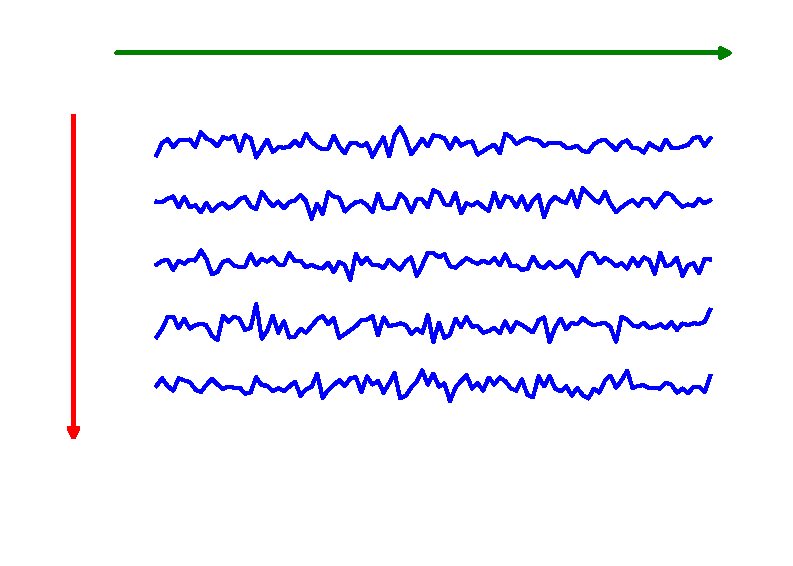
\includegraphics[width=1.2\textwidth]{./chapter_coins/figs/sp_grid.pdf}}
  \put(13,190){$Y_{z_1}(\t)$}
  \put(13,159){$Y_{z_2}(\t)$}
  \put(13,128){$Y_{z_3}(\t)$}
  \put(13,97){$Y_{z_4}(\t)$}
  \put(13,66){$Y_{z_5}(\t)$}
  \put(-20,180){\rotatebox{-90}{realization (universe) $\gi$}}  
%  \put(-25,12){(universe)}  
%  \put(122,220){specific moment in time $\t=\t^*$}  
  \put(200,235){Time $\t$}  
  \put(188,207){$Y_{z_1}(\t^*)$}
  \put(187,208){\vector(-1,-1){15}}
%  \put(-27,125){$\gi=3$}
%  \put(362,127){$\overline{Y}_{x_3}=$}
%  \put(340,114){$\lim_{\t\to\infty}\frac{1}{\t}\int_0^{\t} Y_{x_3}(\gs)\gd \gs$}
%  \put(100,10){$\ave{Y_X(\t^*)}=\lim_{\N\to\infty}\frac{1}{\N}\sum_{i=1}^\N Y_{x_i}(\t^*)$}  
\label{sp_grid}
\end{picture}\\
%\end{figure}
When we simulate stochastic processes, we often start with some value and modify it iteratively, for example in each step of a for-loop. In each step we generate a new instance of a random number and thereby construct the trajectory of the stochastic process. In \eref{st_pr} it's not generated that way. Instead, in this picture, we generate an instance $\z$ of the random variable $\Z$ only once and insert that into \eref{st_pr}. The value $\z$ specifies a simple function of time
\be
\Y_{\z}(\t)=\gf(\z,\t)
\elabel{st_pr_r}
\ee
meaning that all the randomness is contained in $\z$. Once $\z$ is specified, $\Y_{\z}(\t)$ is specified for all time, and we call it a ``realization'' or ``trajectory'' of the stochastic process. Note the use of capital $\Z$ for the random variable in \eref{st_pr} and small $\z$ for a realization of it in \eref{st_pr_r}. As an example you can think of drawing at random a single uniformly distributed real number from the interval $(0,1)$. With probability 1, this number will be irrational and correspond to an infinite sequence of random decimal digits, which can be interpreted as a stochastic process, where $\t$ is given by the decimal place of the digit.

We can also do this: fix a specific time, $\t^*$, and consider the stochastic process at that time, $\Y_{\Z}(\t^*)$. That's again a random variable, an instance of which may be $\Y_{\z_1}(\t^*)$.

Just as a function of a random variable is another random variable, a function of a stochastic process is another stochastic process. We will often use the noun ``observable'' to refer to a quantity that is derived from a stochastic process. For example, the growth rate of wealth is an observable of the wealth process.

We will suppress the random variable $\Z$ in our notation, and just write $\x(\t)$ for the stochastic wealth process (instead of writing $\x(\Z,\t)$, {\it c.f.} \eref{st_pr}). We will also write $\x(\t)$ for a specific realization of this process, or $\x_\gi(\t)$ when it's important to distinguish different realizations.
\end{excursion}

We pretended to be mathematically clueless when we ran the simulations,
with the purpose to gain a deeper conceptual understanding of the expectation 
value. We now compute exactly the expectation value of the stochastic process $\x(\t)$, instead of 
approximating it numerically. Consider the expectation value of \eref{gamble}  
\be
\ave{\x(\t+\dt)}=\ave{\x(\t)\gr(\t+\dt)}.
\elabel{step_1}
\ee
We've just learned what to call objects like $\gr(\t)$: it's another stochastic process, or an observable. This one is  especially simple: in a given realization $\x(\t)$ it's one instance of the same random variable for each time $\t$.  one, namely one that is ergodic. We note here that its ensemble average is time-independent (and in \secref{Ergodic_observables} we will see that it's an example of an ergodic observable).
Since $\gr(\t+\dt)$ is independent of $\x(\t)$, \eref{step_1} can be re-written as
\be
\ave{\x(\t+\dt)}=\ave{\x(\t)}\ave{\gr}.
\ee
Therefore, we can solve recursively for the wealth after $\T$ rounds, corresponding to a playing time of $\Dt=\T\dt$:
\be
\ave{\x(\t+\Dt)} = \ave{\x(\t+\T\dt)}=\x(\t)\ave{\gr}^\T.
\ee
$\dt$ is the duration of a single round of a gamble, while $\Dt$ is the amount of time spent gambling.

The expectation value $\ave{\gr}$ is easily found from \eref{law} 
as $\ave{\gr}=\frac{1}{2}\times 0.6 + \frac{1}{2}\times 1.5=1.05$. Since 
this number is greater than one, $\ave{\x(\t)}$ grows exponentially in 
time by a factor 1.05 each time unit, or expressed as a continuous 
growth rate, at $\frac{1}{\dt}\ln \ave{\gr}\approx4.9\%$ per time 
unit. This is what might have led us to
%We could now conclude that the case is closed: mathematics 
%tells us that there's some risk involved, but the broad effect of subjecting 
%our wealth to the rules of the game is a gain, and 
conclude that the gamble is worth taking. \Fref{cf_exp} compares the
analytical result for the infinite ensemble to the numerical results 
of \fref{1_2} for finite ensembles.

\begin{figure}[h!]
\begin{picture}(200,200)(0,0)
    \put(-100,0){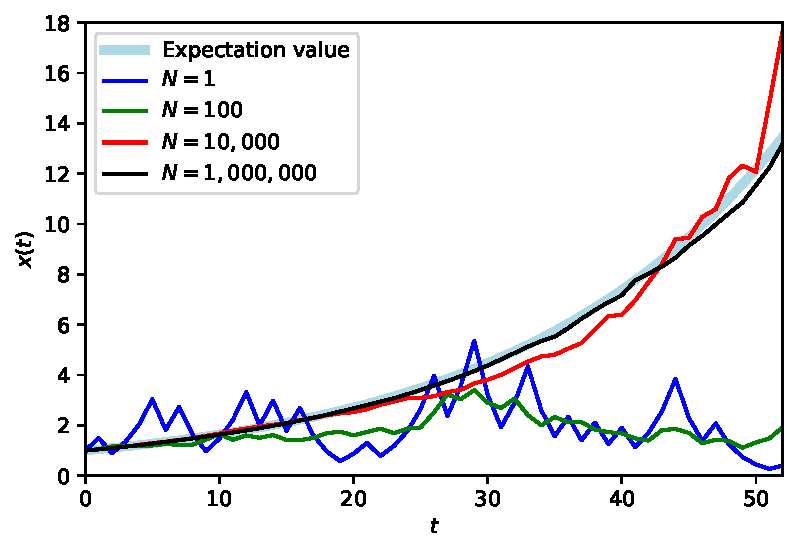
\includegraphics[width=0.8\textwidth]{./chapter_coins/figs/x_of_t_lin_exp.pdf}}
  \put(180,0){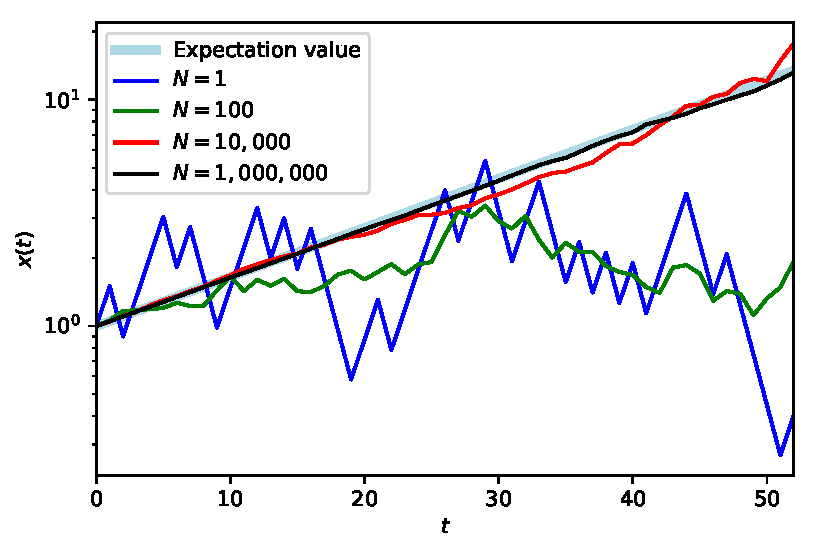
\includegraphics[width=0.8\textwidth]{./chapter_coins/figs/x_of_t_log_exp.pdf}}
  \put(35,160){(A)}
  \put(315,160){(B)}  
\end{picture}
\caption{Expectation value (thick light blue line) and finite-ensemble averages.
 (A) linear scales, (B) logarithmic scales.}
\flabel{cf_exp}
\end{figure}
\FloatBarrier


%But we caution against this. We have correctly computed
%the expectation value, first numerically and then analytically.
We stress that the expectation value is just some mathematical
object -- someone a long time ago gave it a suggestive 
name, but we certainly shouldn't 
give any credence to a statement like ``we expect to find $\x(\t)=\ave{\x(\t)}$ 
because it's the expectation value.'' Mathematical objects
are quite indifferent to the names we give them.


\begin{history}{The invention of the expectation value}
Expectation values 
were not invented in order to assess whether a gamble is 
worth taking. Instead, they were developed to settle a  
moral question that arises in the following somewhat contrived 
context: imagine playing a game of dice with a 
group of gamblers. The rules of the game are simple: we 
roll the dice three times,  and whoever rolls the most points 
gets the pot to which we've all contributed equal amounts. 
We've already rolled the dice twice when suddenly the 
police burst in because they've heard of our illegal gambling ring. 
We all avoid arrest, most of us escape through the backdoor, 
and to everyone's great relief you had the presence of mind 
to grab the pot before jumping out of a conveniently located 
ground-floor window. Later that day, under the cover of dusk, 
we meet behind the old oak tree just outside of town to split 
the pot in a fair way. But hold on -- what does ``fair'' mean here?
Some of us had acquired more points than others in the first 
two rolls of the dice. Shouldn't they get more? The game was 
not concluded, so wouldn't it be fair to return to everyone his 
wager and thank our lucky stars that we weren't arrested? 
Should we split the pot in proportion to each player's points? 
All of these solutions were proposed \cite{Devlin2008}.
The question is fundamentally moral, and there is no 
mathematical answer. But \person{Blaise Pascal}, now famous for 
addressing theological questions using expectation values, put the 
problem to Pierre de Fermat, and over the course of a few months' 
correspondence (the two never met in person) \person{Fermat} and 
\person{Pascal} agreed that fairness is achieved as follows: 
think of all (equally likely) possible outcomes of the third round 
of throws of the dice, call the number of all possibilities $\N$. 
Now count those possibilities that result in player $\gj$ winning, 
call this $\gn_\gj$. If $\q$ is the amount of money in the pot, then 
we split the pot fairly by giving each player
 $\frac{\gn_\gj}{\N}\times \q$.
This is $\ave{\q}$, according to \eref{exp_sum}, 
because $\frac{\gn_\gj}{\N}=\p_\gj$ is the probability that player $\gj$ wins the
amount \q. 
Later researchers called this amount the ``mathematical expectation''  
or simply ``expectation value''. But this is really an unfortunate choice 
 -- no player ``expected'' to receive $\ave{\q}$. 
Instead, each player expected to receive either nothing or $\q$. 
\end{history}

\subsubsection{Time average}
In this section we validate \fref{1_3} and compute analytically 
what happens in the long-time limit. The blue line in \fref{1_3} is not completely smooth, there's still 
some noise (see panel B). It has some average slope, but that slope will vary from realisation to 
realisation. The longer we observe the system, \ie the more time
is represented in a figure like \fref{1_3}, the smoother the line will be. In the long-time limit, $\Dt\to\infty$, 
the line will be completely smooth, and the average slope will be a deterministic number -- in any
realization of the process it will come out identical. 

The dynamic is set up such that wealth at time $\t+\Dt$, where $\Dt=\T\dt$ as before, is
\be
\x(\t+\Dt)=\x(\t)\prod_{\gtau=1}^\T \gr(\t+\gtau\dt),
\ee
with the dummy variable $\gtau$ indicating the round of the game. We can split this into two products, one for each possible value of $\gr(\t)$, which we call
$\gr_1$ and $\gr_2$, \ie
\be
\gr(\t) = \begin{cases}
\gr_1 &\text{with probability } \p_1 \\
\gr_2 &\text{with probability } \p_2 = 1-\p_1.
\end{cases}
\ee
Let's denote the number of occurrences of $\gr_1$ by $\gn_1$ and of $\gr_2$ by $\gn_2$, 
so that
\be
\x(\t+\Dt)= \x(\t)\gr_1^{\gn_1} \gr_2^{\gn_2}.
\ee
% There was confusion here between per-round and per-unit-time wealth multipier. I've changed everything to be consistent with per round (i.e. \T^th root of product as opposed to \Dt^th root) since this is more consistent with the text.
We denote by $\rt$ the effective factor by which $\x(\t)$ is multiplied per round when the change is computed over a long time, \ie $\x(\t+\Dt) \sim\x(\t)(\rt)^\T$ as $\Dt\to\infty$. This quantity is found by taking the $\T^{\text{th}}$ root of $\frac{\x(\t+\Dt)}{\x(\t)}$ and considering its long-time limit:
\bea
\rt &=&\lim_{\Dt\to\infty }\left(\frac{\x(\t+\Dt)}{\x(\t)}\right)^{1/T}\\
 &=& \lim_{\T\to\infty } \gr_1^{\gn_1/\T}\gr_2^{\gn_2/\T}.
\eea
Identifying $\lim_{\T\to\infty} \gn_1/\T$ as the probability 
$\p_1$ for $\gr_1$ to occur (and similarly $\lim_{\T\to\infty}\gn_2/\T=\p_2$) this is
\be
\lim_{\T\to\infty }\left(\frac{\x(\t+\T\dt)}{\x(\t)}\right)^{1/\T}= (\gr_1 \gr_2)^{1/2},
\elabel{long_t}
\ee
or $\sqrt{0.9}\approx 0.95$, \ie a number smaller than one, reflecting 
decay in the long-time limit for the individual trajectory.
The trajectory in \fref{1_3} was not a fluke: {\it every} trajectory
will decay in the long run at a rate of $(\gr_1 \gr_2)^{1/2}$ per round. 

\Fref{1_4} (B) compares the trajectory generated in \fref{1_3} to a trajectory decaying exactly 
at rate $\rt$ and places it next to the average over a million systems.
\begin{figure}[h!]
\begin{picture}(200,200)(0,0)
    \put(-100,0){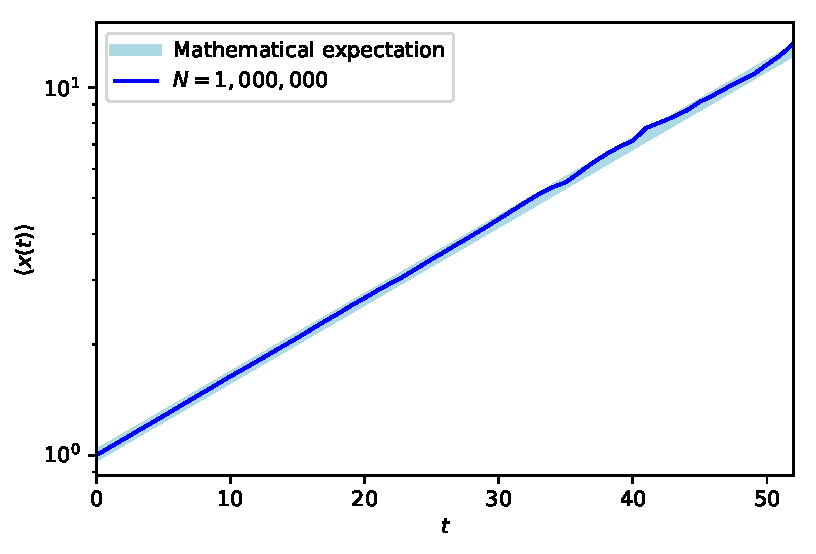
\includegraphics[width=0.77\textwidth]{./chapter_coins/figs/x_of_t_N1M.pdf}}
  \put(180,0){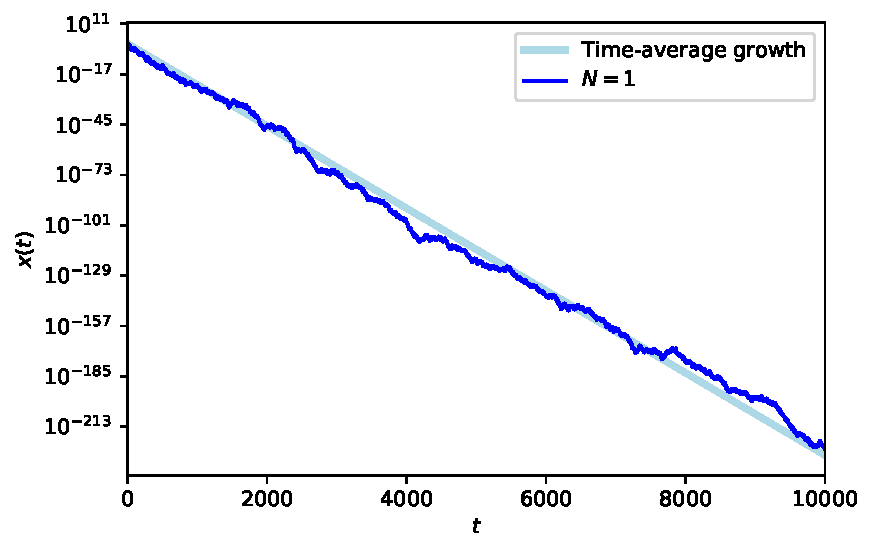
\includegraphics[width=0.8\textwidth]{./chapter_coins/figs/x_of_t_log_10000.pdf}}
  \put(-30,120){(A)}
  \put(250,120){(B)}  
\end{picture}
\caption{(A) Finite-ensemble average for $N=10^6$ and 52 time steps, the light blue line is 
the expectation value.
 (B) A single system simulated for 10,000 time steps, the light blue 
line decays exponentially with the time-average decay factor $\rt$ in each time step.}
\flabel{1_4}
\end{figure}
\FloatBarrier
%\footnotetext{In \fref{1_4} (A) 
%a slight discrepancy between the expectation value and the $\N=10^6$ 
%finite-ensemble average is visible, especially for later times. This is not coincidence --
%in the long run, also the finite-ensemble average for $10^6$ systems will decay
%at the time-average growth rate. A simple proof for this for the continuous process 
%is in \cite{PetersKlein2013}.
%Moreover, much is known about the distribution for $\ave{\x(\t)}_\N$ for 
%any $\N$ and $\t$ (because
%it happens to be mathematically identical to the partition function of the random 
%energy model, introduced and solved by \person{Derrida} \cite{Derrida1980}. We thank 
%\person{J.-P. Bouchaud} for pointing this out to us).}
%\FloatBarrier

\begin{excursion}{Scalars}

$\gr(\t)$ is a random variable, whereas both $\rex$ and $\rt$ are scalars.
Scalars have the so-called ``transitive property'' that is heavily relied upon in 
economic theory. Let $\ga_i$ be a set of scalars. Transitivity means that if $\ga_1>\ga_2$ and 
$\ga_2>\ga_3$ we have $\ga_1>\ga_3$. Notice that we cannot rank random variables 
in such a way. The ``greater than'' relation, $>$,
is not defined for a pair of random variables, which is the mathematical
way of saying that it is difficult to choose between two gambles, and it is why 
we went to the trouble of removing the randomness from the stochastic process 
$\x(\t)$. Removing randomness by
averaging always involves a limiting process, and results are said to hold ``with probability one''. 
In the case of $\rex$ we considered the infinite-ensemble limit, $\N\to \infty$, and 
in the case of $\rt$ we considered the infinite-time limit, $\Dt\to\infty$. If we use the scalars 
$a_i$ to represent preferences, we can test for consistency among preferences. 
For instance, in such a model world where preferences are represented by scalars, 
the facts that ``I prefer kangaroos to Beethoven'' and ``I prefer mango chutney to kangaroos'' 
imply the fact ``I prefer mango chutney to Beethoven''. Translating back to reality, 
economists like to call individuals who make the first two statements but not the 
third ``irrational.'' 

Because transitivity makes for a
nicely ordered world, it is useful to find scalars to represent preferences.
We are skeptical about the attempt to map all preferences
into scalars because  the properties of mango chutney are too different, {\it qualitatively},
from the properties of Beethoven. We will restrict our analysis to money --
the amount of money we will receive is random and this introduces
a complication, but at least we know how to compare one amount to 
another in the limit of no randomness -- there is no qualitative differences 
between $\$1$ and $\$3$, only a quantitative difference. 

Both $\rex$ and $\rt$ are scalars, and both are therefore potentially powerful 
representations of preferences. Your decision whether to accept our gamble could
now be modelled as a choice between the value of the scalar $\rt$ if you do not
accept our game, namely $\ga_1=1$, and the value of the scalar $\rt$ if you do accept, 
namely approximately $\ga_2=0.95$. In this model of your decision-making you 
would prefer not to play because $1>0.95$.

\end{excursion}

There are two averages, $\rex$ and $\rt$ that we have determined numerically and analytically. 
Neither average is ``wrong'' in itself; instead each average corresponds to a different property
of the system. Each average is the answer to a different question. Saying that ``wealth 
goes up, on average'' is clearly meaningless and should be countered with the question 
``on what type of average?'' 


\begin{history}{William Allen Whitworth}

$\rex$ and $\rt$ are two different properties of the game. $\rex$ is 
the large-ensemble limit, $\rt$ is the long-time limit, of wealth growth it induces. The Victorian 
mathematician William Allen Whitworth postulated $\rt$ as the relevant property 
for an individual deciding whether to take part in a repeated gamble. 
He used this knowledge to write an appendix  entitled ``The disadvantage 
of gambling'' to the 1870 edition of his book ``Choice and Chance'' 
\cite{Whitworth1870}. He phrased his argument in terms of the difference of two squares. 
Imagine that you either win or lose, with equal probability, 
an amount $\epsilon \x(\t)$ in each round of a game. In the long run, positive and 
negative changes will occur equally frequently, and to determine
the overall effect we just need to consider the effect of one positive and one negative change
in a row. Over one up and one down-move wealth changes by the factor
\be
(1+\epsilon)(1-\epsilon)=1-\epsilon^2.
\elabel{Whitworth}
\ee
This factor is clearly less than one, meaning that what's often called a ``fair gamble'' -- one 
that does not change the expectation value of the gambler's wealth -- leads to an 
exponential decay of his wealth over time. Hence the title of the appendix 
``The disadvantage of gambling.'' We will see in \secref{Geometric_Brownian} that Whitworth's work
captured the essence of \Ito's famous 1944 discovery \cite{Ito1944} that was to form the basis of
much of financial mathematics.

Whitworth was arguing against a dogma of expectation values of wealth, that had 
been established almost immediately following Fermat and Pascal's work. He 
hoped to show mathematically that gambling may not be a good idea even if 
the odds are favourable, and was a 
proponent of the notion that commerce should and does
consist of mutually beneficial interactions rather than one winner and one loser. 
In the end his voice was not heard in the economics community. His main career was as a priest at All Saints Church in London's Margaret Street, only a 22 minute stroll away from the (first office of the) London 
Mathematical Laboratory, according to Google \fref{all_saints}.
%
%$\rex$ and $\rt$ are two different properties of the game. $\rex$ is 
%the large-ensemble limit, $\rt$ is the long-time limit. The Victorian 
%mathematician William Allen Whitworth was aware that $\rt$ is often the property 
%relevant for an individual deciding whether to take part in a repeated gamble. 
%He used this knowledge to write an appendix  entitled ``The disadvantage 
%of gambling'' to the 1870 edition of his book ``Choice and Chance'' 
%\cite{Whitworth1870}. His argument, in slightly different notation, went as 
%follows. Imagine that you either win or lose, with equal probability, 
%an amount $\x(\t) \gsigma \sqrt{\dt}$ in each round of a game. This scaling in $\dt$
%is not arbitrarily chosen -- it would be observed if the multiplicative increment in each time interval
%were the product of many independent smaller multiplicative 
%increments, $\ln \gr=\sum_\gi \ln \tilde{\gr_\gi} \tilde{\dt}$. In the long run, positive and 
%negative changes will occur equally frequently, and to determine
%the overall effect we just need to consider the effect of one positive and one negative change
%in a row. Wealth changes by the factor
%\be
%(1+\gsigma \sqrt{\dt})(1-\gsigma \sqrt{\dt}).
%\ee
%We take the square root of this factor to determine what happens time-averaged per 
%round. This is 
%\be
%[(1+\gsigma \sqrt{\dt})(1-\gsigma \sqrt{\dt})]^{1/2}= (1-\gsigma^2 \dt)^{1/2}
%\ee
%Letting $\dt$ become infinitesimal we replace it by $\gdt$, and 
%the first term in a Taylor expansion becomes exact. We find
%\be
%\left[(1+\gsigma \sqrt{\dt})(1-\gsigma \sqrt{\dt})\right]^{1/2}\to 1-\frac{\gsigma^2}{2} \gdt.
%\ee
%We choose this notation (also in \secref{Geometric_Brownian}) to anticipate \Ito's 
%work of 1944 that is now the basis of much of financial mathematics.
%
%Whitworth was arguing against a dogma of expectation values of wealth, that had 
%been established almost immediately following Fermat and Pascal's work. He 
%hoped to show mathematically that gambling may not be a good idea even if 
%the odds are favourable, and was a 
%proponent of the notion that commerce should and does
%consist of mutually beneficial interactions rather than one winner and one loser. 
%In the end his voice was not heard in the economics
%or mathematics communities. He quit mathematics to become a priest at All Saints Church
%in London's Margaret Street, only a 22 minute stroll away from the London 
%Mathematical Laboratory, according to Google.
\end{history}
\begin{figure}[h!]
\begin{picture}(200,270)(0,0)
  \put(-30,0){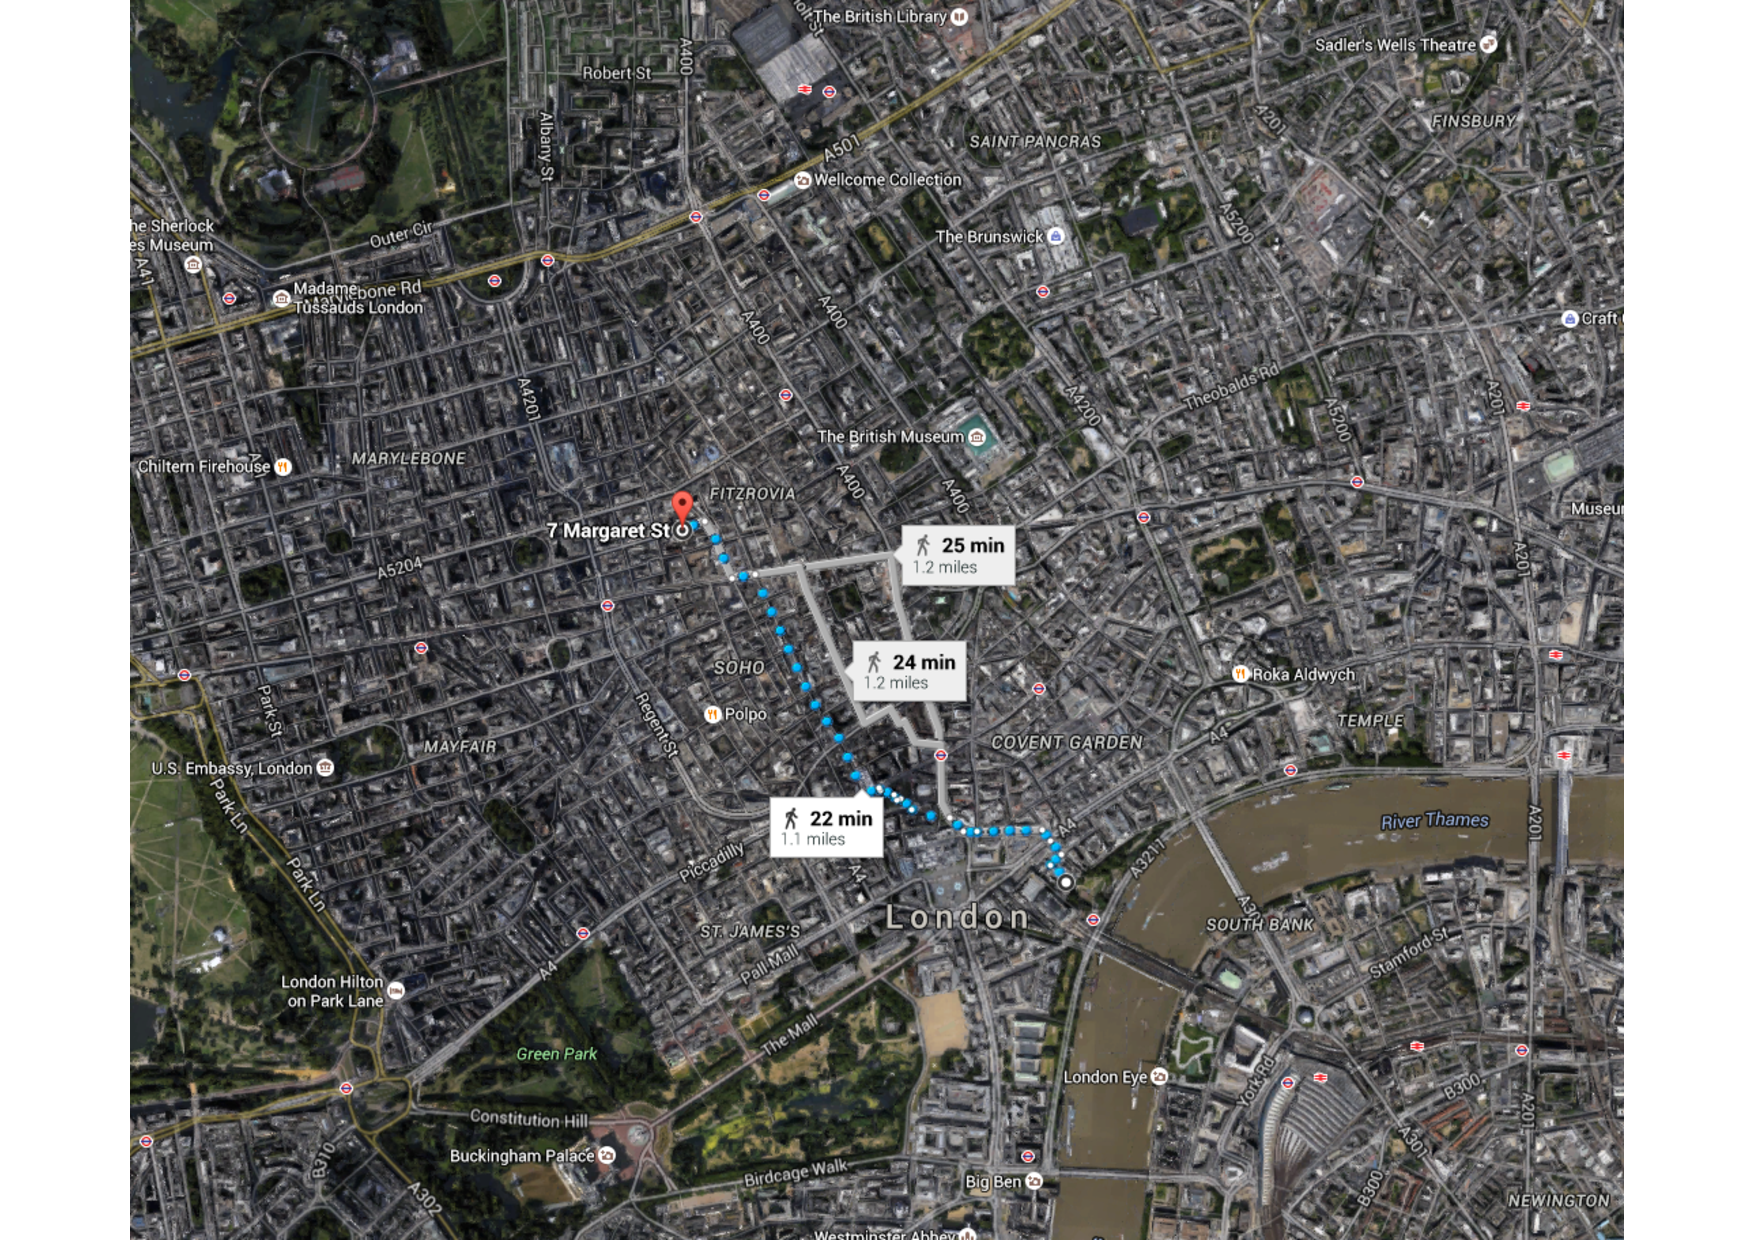
\includegraphics[width=1.15\textwidth]{./chapter_coins/figs/all_saints.pdf}}
\end{picture}
\caption{Location of All Saints Church and the London Mathematical Laboratory's initial office.}
\flabel{all_saints}
\end{figure}
\FloatBarrier


An observable that neatly captures the two different 
aspects of multiplicative growth we have illustrated is the exponential growth rate, $\gm(\ave{\x(\t)}_\N, \Dt)$ 
observed over finite time $\Dt$, in a finite ensemble
of $\N$ realisations. Exponential growth rates are ubiquitous and may be familiar, but because they are the origin of the logarithmic function, which will be important for us later on, we will intro them properly in a little excursion that will also clarify what a logarithm is.

\begin{excursion}{Growth rates, exponentials, and the logarithm}
The logarithm is a relatively recent mathematical discovery, made some time in the 1590s by John Napier, the 8th Laird of Merchiston in Scotland. Let's say you lend me some money, $\x(\t)$, for one year, $\Dt=1$~year, and I have to pay interest on the loan. We agree a yearly interest rate of $r_{1}=5\%$ per year. 

After one year the amount I have to repay is
\bea
\x(\t+\Dt)=\overbrace{\x(\t)}^{\text{Principal}}+ \overbrace{\D \x}^{\text{Interest}}.
\eea 
I could convert the interest payment into a rate, $r_1$, so that $r_1 \x(\t)$ is the rate (dollars per time) at which I have to make constant payments to you for one year, so that you end up with the right amount of interest at the end of the year, and
\be
\x(\t+\Dt)=\x(\t)r_1 \Dt
\elabel{deal}
\ee
This makes it easy, for instance, to find something to enter into my accounts if I have to say after 6 months how much I owe you at that moment. I would say: only half a year has passed, so I only owe you half the interest, 
\be
\x(\t+\Dt/2)=\x(\t)\left(1+r_1 \frac{\Dt}{2}\right). 
\elabel{deal_2}
\ee
But if this is really the amount I owe you after 6 months, surely I should pay interest on this new amount for the following 6 months. We will see that this leads to a problem. Substituting $\x(\t+\Dt/2)$ for $\x(\t)$ on the \RHS of \eref{deal_2} gives
\bea
\x(\t+\Dt)&=&\x(t+\Dt/2)\left(1+r_1 \frac{\Dt}{2}\right)\\
&=&\x(\t)\left(1+r_1\frac{\Dt}{2}\right)^2
\eea
Equating to \eref{deal} we find a contradiction
\bea
\x(\t) (1+ r_{\Dt} \Dt)&=&\x(\t)(1+r_{\Dt}/2)^2\\
\implies 1+ r_{\Dt} \Dt&=&1+r_{\Dt}\Dt+\left(\frac{r\Dt}{2}\right)^2 \text{{\color{red} \huge \lightning}}.
\eea
Strange as it may seem, the solution to this problem is to acknowledge that interest rates depend on the time scale at which they're defined. We can fix the problem by introducing $r_2$ -- the semi-annual interest rate (the subscript 2 indicates that we've split the original interval in 2 equal parts). It is defined by
insisting that the one-step and two-step computations give the same interest payment $\D\x$, 
\be
1+ r_1 \Dt=\left(1+r_2 \frac{\Dt}{2}\right)^2.
\ee
There's nothing stopping us from writing down the general expression for any number, $\T$, of intermediate stock-takings
\bea
\frac{\x(\t+\Dt)}{\x(\t)}&=&\left(1+r_\T\frac{ \Dt}{\T}\right)^\T\\
&\text{which implies}&\\
r_\T&=& \frac{1}{\Dt}\T \left\{\left[\frac{\x(\t+\Dt)}{\x(\t)}\right]^{1/\T}-1\right\}
\eea
A common trick to remove the dependence of some quantity ($r_{\T})$ on another ($\T$)  is to let the control variable diverge. The limit no longer depends on the diverging quantity (we've seen this trick before: the expectation value doesn't depend on the ensemble size, which has diverged).
\be
r_\infty= \frac{1}{\Dt} \underbrace{\lim_{\T\to\infty}\T \left\{\left[\frac{\x(\t+\Dt)}{\x(\t)}\right]^{1/\T}-1\right\}}_{\ln\left(\frac{\x(\t+\Dt)}{\x(\t)}\right)}.
\ee
Note the procedure here: we keep the total time interval, $\Dt$, fixed and split it into $\T$ ever more numerous and shorter sub-intervals $\dt$.
Because it's tedious to write down the long expression involving the limit, we define it as a new function, called the logarithm, $\ln(\cdot)$, as indicated by the underbrace.
\be
\ln \ga :=  \lim_{\T\to\infty}\T \left\{\ga^{1/\T}-1\right\}.
\ee
The logarithm has a property that makes it uniquely suited for characterizing multiplicative processes: the logarithm of a ratio is the difference of the logarithms of numerator and denominator, 
\be
\ln \frac{\ga_2}{\ga_1}=\ln \ga_2 - \ln \ga_1 = \D \ln \ga.
\ee
The inverse function of the logarithm is the exponential, denoted $\exp(\cdot)$, so that $\exp(\ln \ga)=\ga$, and the limiting growth rate $r_\infty$ is called the logarithmic or exponential growth rate, which we also denote by $\gm$ (subscript ''m'' for ``multiplicative'').
\end{excursion}

The exponential growth rate of average wealth in an ensemble of $\N$ systems, observed over time $\Dt$ is
\be
\gm(\ave{\x(\t)}_\N, \Dt)=\frac{\D \ln \ave{\x}_\N}{\Dt},
\elabel{gest}
\ee
where the $\D$ in the numerator corresponds to the change over the $\Dt$ in the denominator. For $\N$ and $\Dt$ finite this is a random variable. The relevant scalars arise as two different limits
of the same stochastic object. The exponential growth rate of the expectation value 
(that's also $\frac{1}{\dt} \ln \ave{\gr}$) is
\be
\gex=\lim_{\N\to\infty}\gm,
\ee
and the exponential growth rate followed by every trajectory when
observed for a long time (that's also $\frac{1}{\dt} \ln \rt$) is 
\be
\gt=\lim_{\Dt\to\infty}\gm.
\elabel{gt}
\ee
We can also write \eref{gest} as a sum of the logarithmic differences in  the 
$\T$ individual rounds of the gamble that make up the time interval 
$\Dt=\T \dt$
\be
\gm(\ave{\x(\t)}_\N, \Dt)=\frac{1}{\T\dt}  \sum_{\gtau=1}^{\T} \D\ln \ave{\x(\t+\gtau\dt)}_\N.
\ee
%For a single trajectory, $\N=1$, \eref{gt} becomes
%\bea
%\t&=&\lim_{\t\to\infty}\frac{1}{\t} \ln \x(\t)\\
%&=&\lim_{\T\to\infty}\frac{1}{\T\dt} \sum_\t^\T \D \ln \x(\t).
%\eea
This leads us to a technical definition of the time average.

\begin{defn}{Finite-time average}
The ``finite-time average'' of the quantity $\x(\t)$ is
\be
\xbar_{\Dt}=\frac{1}{\Dt}\int_{\t}^{\t+\Dt} \x(\gs)\gd\gs.
\elabel{t_ave_f}
\ee
If $\x$ only changes at $\T=\Dt/\dt$ discrete times 
$\t+\dt$, $\t+2\dt$, {\it etc.}, then this can be written as 
\be
\xbar_{\Dt}=\frac{1}{\T\dt}\sum_{\gtau=1}^{\T}\x(\t+\gtau \dt).
\elabel{t_ave_f_disc}
\ee
\end{defn}

\begin{defn}{Time average}
The ``time average'' is the long-time limit
of the finite-time average
\be
\xbar=\lim_{\Dt\to\infty}\xbar_{\Dt}.
\elabel{t_ave}
\ee
\end{defn}
According to this definition, $\gt$ is the time average of 
the observable $\frac{\d \ln \x}{\dt}$. It can be shown that
the time-average growth rate of a single trajectory is the same as that
of a finite-ensemble average of trajectories,
$\lim_{\Dt\to\infty}\frac{\D \ln \x}{\Dt}=\lim_{\Dt\to\infty}\frac{\D \ln \ave{\x}_N}{\Dt}$, \cite{PetersKlein2013}. In \secref{finite_populations} we will derive this result as well as growth rates in finite ensembles and finite time.


\begin{excursion}{Dimensional analysis}
We will often and without qualm write the expression $\D \ln \x$. Dimensional
analysis suggests to think about this expression carefully, at least once. This may
seem pedantic but the absence of this pedantry has caused sufficient
confusion in economic theory for us to risk antagonizing you. ``Dimension'' in this context is closely related to the 
concept of ``unit'' -- for instance, a dollar is a money unit, and the dimension function
for money tells us how to convert from one currency into another. Similarly, length may 
have the unit ``meter'', and the dimension function for length tells us how to convert between 
different systems of units, such as meters and yards. 
We can only point to the subject here and recommend the book
by \person{Barenblatt} for a comprehensive treatment \cite{Barenblatt2003}.
Dimensional analysis is a deeply fascinating and powerful tool that every physicist 
is drilled to use at all times. \person{Taylor} famously used it to compute the energy
released by an early nuclear explosion at the Trinity site near Alamogordo, New Mexico, based on 
some grainy pictures published by Life magazine, at least that's the legend 
\cite{Taylor1950b,Deakin2011}. Fluid dynamicists in general use it to find meaningful quantities 
to distinguish different types of flow. In many problems involving random walks dimensional 
analysis immediately reveals scaling properties, supposed solutions to many problems can
be seen at a glance to be wrong, and, conversely some complicated-looking 
problems can be solved as if by magic just by appealing to dimensional analysis.

\person{Barenblatt} shows in his book that the dimension function must be a (scale-free) power-law 
monomial if there is to be no distinguished system of units. We can all agree that the unit
of money is physically irrelevant -- I can do exactly the same with the pennies in my 
bank account as I can do with the pounds those pennies correspond to. Since this is so, 
for functions of monetary amounts to be physically meaningful we want them to be 
power-law monomials. An amount of square-dollars, $\$^2$, may be meaningful, but an
amount of logarithmic or exponential dollars cannot be meaningful. Hence $\ln(\x)$ on its own
is just some symbol spat on a page by a printer, but it has no physical meaning.
The reason we're comfortable writing $\D \ln \x$ is the unique property of the logarithmic function
\be
\ln \x_1 - \ln \x_2 = \ln\left(\frac{\x_1}{\x_2}\right).
\ee
The quantity in brackets on the \RHS is always dimensionless, it's a pure number because
the dimension functions of two different values of $\x$ always cancel out. So do the units:
$\$1/\$2=1/2$, which is a pure number without units. We will see that indeed only differences 
in logarithms of $\x$ will appear in these lecture notes or in any other reasonable lecture notes. 
Pedantically, we would refuse to write $\D \ln(\x)$ and insist on writing $\ln\left(\frac{\x_1}{\x_2}\right)$.
Since the first notation is shorter and one can make formal arguments for its validity, we are 
happy to use it here. 

The issue is related to a result obtained by \person{von Neumann} and 
\person{Morgenstern} in their 
famous
%but quite unhelpful
book \cite{vonNeumannMorgenstern1944}: 
only differences in utility functions can have physical meaning. 
We will have a lot more to say about utility functions (which we call ergodicity mappings) in \cref{decision}.
\end{excursion}

\subsubsection{Ergodic observables}
\seclabel{Ergodic_observables}

We have encountered two types of averaging -- the ensemble average and the
time average. In our case -- assessing whether it will be good for you to play our 
game, the time average is the interesting quantity because it tells you what happens
to your wealth as time passes. The ensemble average is irrelevant 
because you do not live your life as an ensemble of many yous who can average
over their wealths. Whether you like it or not, you will experience yourself owning 
your own wealth at future times; whether you like it not, you will never experience
yourself owning the wealth of a different realization of yourself. The different realizations,
and therefore the expectation value, are fiction, fantasy, imagined.

We are fully aware that it can be counter-intuitive that with probability one, a different
rate is observed for the expectation value than for any trajectory over time. It sounds
strange that the expectation value is completely irrelevant to the problem. A reason
for the intuitive discomfort is history: since the 1650s we have been trained to
compute expectation values, with the implicit belief that they will reflect what happens
over time. It may be helpful to point out that all of this trouble has a name that's well-known
to certain people, and that an entire field of mathematics is devoted to dealing with
precisely this problem. The field of mathematics is called ``ergodic theory.'' It emerged
from the question under what circumstances the expectation value is informative 
of what happens over time, first raised in the development of statistical mechanics by Maxwell and 
Boltzmann starting in the 1850s. These lecture notes are our attempt to use precisely the insights of these physicists to re-develop economic theory from the foundations up.

\begin{history}{Randomness and ergodicity in physics}

The 1850s were about 200 years after \person{Fermat} and \person{Pascal} introduced expectation 
values into the study of random systems. Following the success of \person{Newton}'s 
laws of motion, established around the same time as the expectation value, 
the notion of ``proper science'' had become synonymous with 
mechanics. Mechanics had no use for randomness and probability 
theory, and the success of mechanics was interpreted as a sign that 
the world was deterministic and that sooner or later we would understand 
what at the time still seemed random. At that point probability theory would 
become obsolete. 

When \person{Boltzmann} hit upon the ingenious idea of introducing randomness into 
physics, to explain the laws of thermodynamics in terms of the underlying 
dynamics of large numbers of molecules, he was fighting an uphill battle. 
Neither molecules nor randomness were much liked in the physics 
community, especially in continental Europe, right up until the publication of 
\person{Einstein}'s 1905 paper on diffusion \cite{Einstein1905}. \person{Boltzmann} had to be 
more careful than \person{Fermat} and \person{Pascal}. He had to pre-empt
predictable objections from his peers, and the question of ergodicity had to be 
answered -- the usefulness of probability theory relies heavily on expectation 
values, but as we have seen, they are averages over imagined future states of the 
universe. \person{Boltzmann}'s critics were aware of this and were not shy to voice their
concerns. Under what circumstances are expectation values meaningful? 
\person{Boltzmann} gave two answers. 
\bi
\item expectation values are meaningful when 
the quantity of interest really is an average (or a sum) over many approximately 
independent systems. An average over a finite ensemble will be close to the 
expectation value if the ensemble is large enough. 
\item expectation values 
are meaningful, even if only a single system exists, if they reflect what happens over time. 
\ei

\person{Boltzmann} called a system ``ergodic\footnote{The word ``ergodic'' was coined by \person{Boltzmann}. 
He initially proposed the word ``monodic'', from Greek $\mu o \nu o$ (unique) + $o\delta o \varsigma$ (path) suggesting 
that a single path when followed for a sufficiently long time will explore all there is to explore and reflect what happens 
in an ensemble. The term ``ergodic'' refers to the specific system \person{Boltzmann} was considering, namely an energy 
($\epsilon \rho \gamma o \nu$) shell across which a path is being traced out.}'' if the possible 
states of the system could be assigned probabilities in such a way that
the expectation value of any observable with respect to those probabilities would 
be the same as its time average with probability 1.

Our setup requires us to be more modest, and we will speak of specific ergodic observables (not of ergodic systems) if their ensemble and time averages are the same.
\end{history}

To convey concisely that we cannot use the expectation value and the 
time average interchangeably in our game, we would say ``the observable $\x$ is not ergodic.'' 

\begin{defn}{Ergodic property}
In these notes, an observable $\A$ is called ergodic if its 
expectation value is constant in time
%, $\frac{\gd\ave{\A}}{\gd\t}=0$, 
and its time average converges to this value with probability one\footnote{Some researchers would call $\A$ ``mean ergodic'' and require further observables derived from it to be (mean) ergodic in order to call $\A$ ``wide-sense ergodic.'' This extra nomenclature is not necessary for our work, but we leave a footnote here to avoid confusion.}

\be
\lim_{\Dt \to\infty}\frac{1}{\Dt } \int_{\t}^{\t+\Dt} \A(\gs) \gd\gs =\lim_{\N\to\infty} \frac{1}{\N}\sum_\gi^\N \A_\gi(\t) .
\elabel{def_ergodic}
\ee
\end{defn}
The \RHS of \eref{def_ergodic} is evaluated at time $\t$, and unlike the \LHS could be a function of time. For now, we restrict our definition of ergodicity to a setup where that is not the case, \ie where the ergodic property holds at all times. In \secref{RGBM_moments} we will discuss transient behavior, where the distribution of $\A$ is time dependent. We then also consider an observable ``ergodic'' if its expectation value only converges to the time-average in the $\t\to\infty$ limit.

In terms of random variables, $\Z$, and stochastic processes, $\Y_{\Z}(\t)$, the ergodic property can be
visualized as in \fref{ergodic_grid}. Averaging a stochastic process over time or over the ensemble
are completely different operations, and only under very rare circumstances (namely under ergodicity) can the two operations be interchanged. In our coin-tossing game the operations are clearly not interchangeable. An implicit assumption of interchangeability in the early days is the Original Sin of economic theory.
\begin{figure}[h!]
\begin{picture}(200,260)(0,0)
  \put(-40,-30){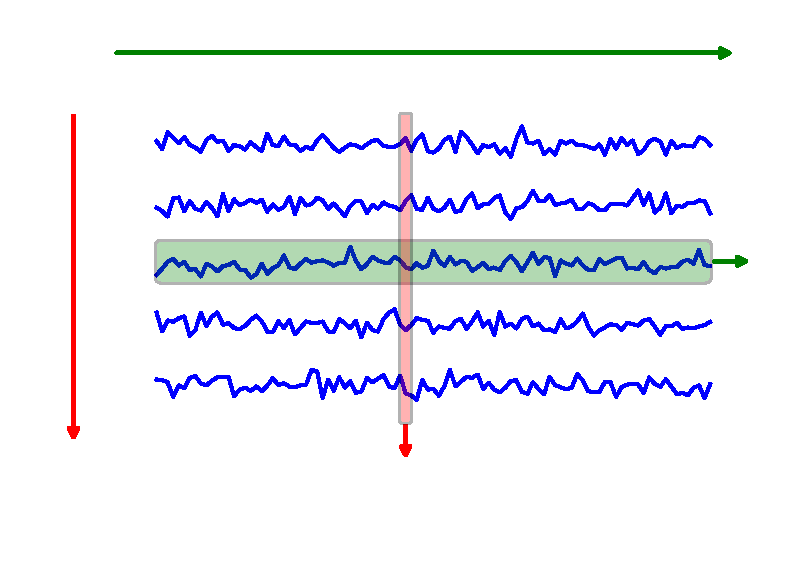
\includegraphics[width=1.2\textwidth]{./chapter_coins/figs/ergodic_grid.pdf}}
  \put(13,190){$\Y_{\z_1}(\t)$}
  \put(13,159){$\Y_{\z_2}(\t)$}
  \put(13,128){$\Y_{\z_3}(\t)$}
  \put(13,97){$\Y_{\z_4}(\t)$}
  \put(13,66){$\Y_{\z_5}(\t)$}
  \put(-25,22){realization}  
  \put(-25,12){(universe) $\gi$}  
  \put(162,242){$\t=\t^*$}  
  \put(344,235){Time $\t$}  
  \put(188,207){$\Y_{\z_1}(\t^*)$}
  \put(187,208){\vector(-1,-1){15}}
  \put(-27,125){$\gi=3$}
  \put(362,127){$\overline{\Y}_{\z_3}=$}
  \put(340,114){$\lim_{\t\to\infty}\frac{1}{\t}\int_0^{\t} \Y_{\z_3}(\gs)\gd \gs$}
  \put(100,10){$\ave{\Y_{\Z}(\t^*)}=\lim_{\N\to\infty}\frac{1}{\N}\sum_{i=1}^\N \Y_{\z_\gi}(\t^*)$}  
\end{picture}
\caption{Extending the figure on p.~\pageref{sp_grid}, averaging over time means averaging 
along one trajectory from left to right; averaging over the ensemble
means averaging at a fixed time across different trajectories from top to bottom.}
\flabel{ergodic_grid}
\end{figure}
%\FloatBarrier

We stress that in a given setup, some observables may have the ergodic property even
if others do not. Language therefore must be used carefully. Saying our game is non-ergodic
really means that some key observables of interest, most notably wealth $\x$, are
not ergodic. Wealth $\x(\t)$, defined by \eref{law}, is clearly not ergodic -- with $\A=\x$ the \LHS of \eref{def_ergodic} 
is zero, and the \RHS is not constant in time but grows. The expectation value $\ave{\x}(\t)$
simply doesn't give us the relevant information about the temporal behavior of $\x(\t)$.
 
This does not mean that no ergodic observables exist that are related
to $\x$. Such observables do exist, and
we have already encountered two of them. In fact, we will encounter a particular type
of them frequently -- in our quest for an observable that tells us what happens over
time in a stochastic system we will find them automatically. However, again, the issue
is subtle: an ergodic observable may or may not tell  us what we're interested in.
It may be ergodic but not indicate what happens to $\x$. For example, 
the multiplicative factor $\gr(\t)$ is an 
ergodic observable that reflects what happens to the expectation value of $\x$, 
whereas per-round changes in the logarithm of wealth, $\d \ln \x = \ln \gr$, are also ergodic 
and reflect what happens to $\x$ over time.

\vspace{.3cm}
\underline{Proposition:} $\gr(\t)$ and $\d \ln \x$  are ergodic for the wealth dynamic defined by \eref{law} and \eref{gamble}.

\begin{proof}

According to \eref{ens} and \eref{f_ens}, the expectation value of $r(t)$ is
\be
\ave{\gr}=\lim_{\N\to\infty} \frac{1}{\N} \sum_\gi^\N \gr_\gi,
\elabel{e_r}
\ee
and, according to \eref{t_ave_f_disc}, the time average of $\gr(\t)$ is
\be
\tave{\gr}=\lim_{\T\to\infty} \frac{1}{\T} \sum_\gtau^\T \gr_\gtau,
\elabel{t_r}
\ee
where we have written $\gr_\gtau = \gr(\t+\gtau\dt)$ to make clear the equivalence between the two expressions. The only difference is between the labels we have chosen
for the dummy variable ($\gi$ in \eref{e_r} and $\gtau$ in \eref{t_r}). Clearly, the 
expressions yield the same value. 

The same argument holds for $\d \ln \x$.
\end{proof}

Whether we consider \eref{t_r} an average over 
time or over an ensemble is only a matter of our choice of words. 

The expectation value $\ave{\d \ln \x}$ is important, historically. \person{Daniel Bernoulli} noticed in 
1738 \cite{Bernoulli1738} that people tend to
optimize $\ave{\d \ln \x}$, whereas it had been assumed that they should optimize $\ave{\d \x}$. 
Unaware of the issue of ergodicity (200 years before the concept was discovered 
and the word was coined), \person{Bernoulli} had no good explanation for this 
empirical fact and simply stated that people tend to behave as though they valued
money non-linearly. We now know what is actually going on: multiplicative dynamics
are a fairly realistic model for real wealth, and under those dynamics
$\d \x$ is not ergodic, 
and $\ave{\d \x}$ is of no interest -- it doesn't tell us what happens over time. However,
$\d \ln \x$ {\it is} ergodic, and $\ave{\d \ln \x}$ does tell us what happens to $\x$ over time, 
wherefore seeing people optimise $\ave{\d \ln \x}$ just means seeing them optimise wealth 
over the one trajectory that describes a financial life, rather than across the ensemble of possibilities.

% repetition
%When the foundations of economic theory were laid, specifically in \person{Bernoulli}'s 
%seminal paper of 1738 \cite{Bernoulli1738}, the distinction between ergodic and
%non-ergodic observables was unknown. Researchers thought that the expectation value
%of $\d \x$ reflected what happens over time but observed that real people behaved
%according to what the expectation value of $\d \ln \x$ would suggest. While the origin of the 
%discrepancy remained mysterious and numerous puzzles and paradoxes in 
%economic theory arose as a result. The paradigm we outline here resolves these puzzles.

Ergodicity is not the same concept as stationarity. As an illustration of the difference, consider the following process: $\gf(\t)=\z_{\gi}$, where $\z_{\gi}$ is an instance of a random variable $\Z$. Explicitly, this means a realisation of the stochastic process $\gf(\t)$ is generated as follows: we generate the random instance $\z_{\gi}$ once, and then fix $\gf(\t)$ at that value for all time. The distribution of $\gf(\t)$ is independent of $\t$ and in that sense $\gf(\t)$ is stationary. But it is not ergodic: averaging over the ensemble, we obtain $\ave{\gf(\t)}=\ave{\z}$, whereas averaging over time in the $\gi^{\text{th}}$ trajectory gives $\overline{\gf}=\z_{\gi}$. Thus the process is stationary but not ergodic.

\subsection{Rates}
\seclabel{Rates}
This section is a preview of an in-depth discussion of growth rates in \cref{decision}.
The ergodic observable $\d \ln \x$, identified in the previous section, is basically a rate.
Dividing it by the duration of the gamble, we obtain exactly the exponential 
growth rate of $\x$, namely $\frac{\d \ln \x}{\dt}$. Finding good growth rates 
will be important, wherefore we now discuss the notion of a rate and 
the notion of time independence. 
To do this properly let's think about the basic task of science. This may be described as the 
search for stable structure. Science attempts to build models of the world 
whose applicability does not vary over time. This doesn't mean that the world doesn't change, 
but the way in which the models describe change does not change. The model identifies
something stable. This is implied by the fact that we can write 
equations (or English sentences) in ink on paper, with the equation (or sentence) remaining 
useful over time. The ink won't change over time, so
if an article written in 1905 is useful today then it must describe something that hasn't 
changed in the meantime. These ``somethings'' are often somewhat 
grandiosely called laws of nature.

\person{Newton}'s laws are a good illustration of this. They are part of mechanics, meaning that they
are an idealized mathematical model of the behavior of positions, time, and masses. 
For instance, \person{Newton}'s second law, $\NF=\Nm \frac{\gd^2 \Nx}{\gd\t^2}$, states that the mass multiplied by 
the rate of change of the rate of change of its position equals the force. The law is an unchanging 
law about positions, time, and masses, but it does not say that positions don't change, it doesn't even say 
that rates of change of positions don't change. It does say that the rate of change of the 
rate of change of a position remains unchanged so long as the force and the mass 
remain unchanged. \person{Newton}'s deep insight was to transform an unstable thing -- the position of a mass --
until it became stable: he fixed the force and considered rates of changes of rates of changes, et 
voil\'a!, a useful equation could be written down in ink, remaining useful for 350 years so far.

Like \person{Newton}'s laws (a mathematical model of the world), our game is a prescription of changes. 
Unlike \person{Newton}'s laws it's stochastic, but it's a prescription of changes nonetheless. 
The multiplicative aspect of our game makes it also a powerful mathematical model of the world, as we shall see in subsequent lectures. 

We're very much interested in changes of $\x$ -- we want to know 
whether we're winning or losing -- but changes in $\x$ are not stable. 
Under the rules of the game the rate of change of wealth, $\frac{\d \x(\t)}{\dt}$, is a different 
random variable for each $\t$ because it is proportional to $\x(\t)$. But not to worry, 
in \person{Newton}'s case changes in the position are not stable either, even in a 
constant force field. Nonetheless \person{Newton} found a useful stable property. 
Maybe we can do something similar. We're looking for a function $\gv(\x)$ that satisfies two conditions: 
it should indicate what happens to $\x$ itself, and its random changes should be instances of a time-independent random variable.

The first condition is that $\gv(\x)$ must tell us 
whether $\x(\t)$ is growing or shrinking -- this just means that $\gv(\x)$ has to 
be monotonic in $\x$. We know that there is something time-independent
about $\x$ because we were able to write down in ink how $\x$ changes. So we only need 
to find the monotonic function of $\x$ whose additive changes inherit the time-independence 
of the ink in \eref{law}. The game is defined by a set of factors of change in $\x(\t)$, \eref{gamble}. 
Therefore, the fractional change in $\x$, namely
$\gr(\t) = \frac{\x(\t+\dt)}{\x(\t)}$, comes from a time-independent distribution. Which 
function responds additively to a multiplicative change in its argument? 
The answer is the logarithm, \ie
only the logarithm satisfies
\be
\gv[\x(\t+\dt)]-\gv[\x(\t)]=\gv \left(\frac{\x(\t+\dt)}{\x(\t)}\right)
\ee
and we conclude that for our game $\gv(\x)=\ln\x$.
For multiplicative dynamics, \ie if $\frac{\x(\t+\dt)}{\x(\t)}$ is stationary, the expectation 
value of the rate of change of the logarithm of $\x(\t)$ determines whether the game is long-term profitable 
for an individual.

More generally, when evaluating a gamble that is represented as a stochastic process, it seems that people's intuitive
choices roughly maximise appropriate long-time growth rates. Mathematically speaking, they
\begin{enumerate}
\item
find a monotonically increasing function $\gv[\x(\t)]$ such that $\frac{\d \gv[\x(\t)]}{\dt}$ 
are independent instances of a stationary random variable.
\item
compute the expectation value of $\frac{\d \gv[\x(\t)]}{\dt}$. If this is positive then $\x(\t)$
grows in the long run, if it is negative then $\x(\t)$ decays.
\end{enumerate}

The mathematics of this procedure is discussed in detail in \cref{decision}, and an
experiment testing whether people behave as predicted is described in \secref{Copenhagen}.

\subsection{Brownian motion}
\seclabel{Brownian_motion}
In the previous section we established that the discrete increments of the logarithm of 
$\x$, which we called $\gv$, are instances of a time-independent random variable in our game. A quantity 
for which this is the case performs a random walk.
Indeed, the blue line for a single system in \fref{1_2} (B) shows 52 steps of a random walk trajectory.
Random walks come in many forms -- in all of them $\gv$ changes discontinuously by an amount 
$\d \gv$ drawn from a time-independent distribution, over time intervals which may be regular or which may be drawn from a time-independent distribution themselves.

We are interested only in the simple case where $\gv$ changes at regular intervals, $\dt, 2\dt, \dots$. For 
the distribution of increments we only insist on the existence of the variance, meaning we insist that 
$\var(\d \gv)=\ave{\d \gv^2}-\ave{\d \gv}^2$ be finite. The change in $\gv$ after a long time is then the sum 
of many independent instances of increments, 
\be
\gv(\t+\T\dt)-\gv(\t)=\sum_\gi^\T \d \gv_\gi.
\ee
The Gaussian central limit theorem tells us that such a sum, properly rescaled, will be 
Gaussian distributed
\be
\lim_{\T\to\infty} \frac{1}{\sqrt{\T}}\sum_\gi^\T \d \gv_\gi -\T\ave{\d \gv} \sim \mathcal{\N}(0 , \var(\d \gv)),
\elabel{CLT}
\ee
where we call $\frac{\ave{\d \gv}}{\dt}$ the drift term. The logarithmic change in the 
long-time limit that was of interest to us in the analysis of the coin toss game is thus 
Gaussian distributed. 

Let's also ask about the re-scaling that was applied in \eref{CLT}. 
Scaling properties are very robust, and especially the scaling  
of random walks for long times will be useful to us. We work with the
simplest setup: we start at zero, $\gv(0)=0$, and in each time step, we either increase or 
decrease $\gv$ by 1, with probability 1/2. 
We are interested in the variance of the distribution of $\gv$ as $\T$ increases, which we obtain by
computing the first and second moments of the distribution. The expectation value (the first moment)
of $\gv$ is $\ave{\gv}(\T)=0$, by symmetry for all times. We obtain the second moment by 
induction\footnote{The argument is nicely illustrated in \cite[Volume 1, Chapter 6-4]{Feynman1963}, 
where we first came across it.}:
Whatever the second moment, $\ave{\gv(\T)^2}$, is at time $\T$, we can write down its value at
time $\T+1$ as 
\bea
\ave{\gv(\T+1)^2}&=&\frac{1}{2}\left[\ave{(\gv(\T)+1)^2}+\ave{(\gv(\T)-1)^2}\right]\\
&=&\frac{1}{2}\left[\ave{\gv(\T)^2+1+2\gv(\T)}+\ave{(\gv(\T)^2+1-2\gv(\T))}\right]\\
&=&\ave{\gv(\T)^2}+1.
\eea
In addition, we know the initial value of $\gv(0)=0$. By induction it follows that the second moment is
\be
\ave{\gv(\T)^2}=T
\ee
and, since the first moment is zero, the variance is
\be
\var(\gv(\T))=T.
\elabel{BM_var}
\ee
The standard deviation -- the width of the distribution -- of changes in a quantity 
following a random walk thus scales as the square-root of the number of steps 
that have been taken, $\sqrt{\T}$. This square-root behaviour leads to many interesting
results. It can make averages stable (because $\sqrt{\T}/\T$ converges to zero for large $\T$), 
and sums unstable (because $\sqrt{\T}$ diverges for large $\T$).

Imagine simulating a single long trajectory of $\gv$ and plotting it on paper\footnote{This argument is
inspired by a colloquium presented by Wendelin Werner in the mathematics department of Imperial 
College London in January 2012. 
Werner started the colloquium with a slide that showed a straight horizontal line and asked: what is this? 
Then answered that it was the trajectory of a random walk, with the vertical and horizontal axes scaled equally.}. 
The amount of 
time that has to be represented by a fixed length of paper increases linearly with the simulated time
because the paper has a finite width to accommodate the horizontal axis. 
If $\ave{\d \gv} \neq 0$ then the amount of variation in $\gv$ that has to be represented by a fixed
amount of paper also increases linearly with the simulated time. However, the departures of $\D\gv$ from
its expectation value $\T \ave{\d \gv}$ only increase as the square-root of $\T$. Thus, the 
amount of paper-space given to these departures scales as $\T^{-1/2}$, and for very long simulated
times the trajectory will look like a straight line on paper.

In an intermediate regime, fluctuations will still be visible but they will also be approximately 
Gaussian distributed. In this regime it is often easier to replace the random walk model 
with the corresponding continuous process. That process is called \BM and is intuitively thought
of as the limit of a random walk where we shorten the duration of a step $\dt \to 0$, and 
scale the width of an individual step so as to maintain the random-walk scaling of the variance, meaning
$|\d\gv|=\sqrt{\dt}$. In the limit $\dt\to0$, this implies that $\frac{\d\gv}{\dt}$ diverges, so \BM trajectories 
are infinitely jagged, or -- in mathematical terms -- they are not differentiable. However, the way in
which they become non-differentiable, though the $\sqrt{\dt}$ factor, leaves the 
trajectories just continuous (this isn't the case for $|\d\gv|=\dt^\alpha$, where $\alpha$ is less than 0.5). 
Continuity of $\gv$ 
means that it is possible to make the difference $|\gv(\t)-\gv(\t+\epsilon)|$ arbitrarily small by choosing
$\epsilon$ sufficiently small. This would not be possible if there was a jump in $\gv(\t)$, so continuity 
roughly means that there are no jumps. These subtleties make \BM a topic of great mathematical
interest, and many books have been written about it. We will pick from these books only what is 
immediately useful to us.
To convey the universality of \BM we define it formally as follows:

\begin{defn}{Brownian motion i}
If a stochastic process has continuous paths, stationary independent increments, and is distributed according to 
$\mathcal{\N}(\gmu \t, \gsigma^2 \t)$ then it is a Brownian motion.
\end{defn}

The process can be defined in different ways. Another illuminating definition is this:

\begin{defn}{Brownian motion ii}
If a stochastic process is continuous, with stationary independent increments, then the process is a Brownian 
motion.
\end{defn}

We quote from \cite{Harrison2013}: {\it ``This beautiful theorem shows that Brownian motion can actually be defined
by stationary independent increments and path continuity alone, with normality following as a consequence 
of these assumptions. This may do more than any other characterization to explain the significance of 
Brownian motion for probabilistic modeling.''}

Indeed, \BM is not just a mathematically rich model but also -- due to its emergence through the Gaussian 
central limit theorem -- a model that represents a large universality class, 
\ie it is a good description of what happens over long times 
in many other models. \BM is a process with two parameters, $\gmu$ and $\gsigma$.
It can be written as a stochastic differential equation
\be
\gd\gv=\gmu \gd\t + \gsigma \gd\gW
\elabel{BM_dx}
\ee
where $\gd\gW$ is a Wiener increment. The Wiener increment can be defined by its distribution and correlator, 
\bea
\gd\gW &\sim& \mathcal{\N}(0,\gd\t)\\
\ave{\gd\gW(\t) \gd\gW(\t')}&=&\gd\t~ \gdelta(\t,\t'),
\eea
where $\gdelta(\t,\t')$ is the Kronecker delta -- zero if its two arguments differ ($\t\neq \t'$), and one if 
they are identical ($\t=\t'$).\footnote{Physicists often write $\gd\gW=\geta \gd\t$, where $\ave{\geta}=0$ and 
$\ave{\geta(\t) \geta(\t')}=\gdelta(\t-\t')$, in which case $\gdelta(\t-\t')$ is the Dirac 
delta function, defined by the integral $\int_{-\infty}^{\infty} \gf(\t) \gdelta(\t-\t') \gd\t=\gf(\t')$. Because of its singular
nature ($\geta(t)$ does not exist (``is infinite''), only its integral exists) it can be difficult to develop
an intuition for this object, and we prefer the $dW$ notation.} The notation $\sim \mathcal{N}(0, \gd\t)$ is short-hand for ``is Gaussian distributed, with mean $0$ and variance $\gd\t$.''
In simulations \BM paths can be constructed from a discretized version of \eref{BM_dx}
\be
\gv(\t+\dt)=\gv(\t)+ \gmu \dt + \gsigma \sqrt{\dt} \gxi_\t,
\ee
where $\gxi_\t$ are instances of a standard normal distribution.

\BM itself is not a time-independent random variable -- it is a non-ergodic stochastic process. This is easily seen
by comparing expectation value and time average
\be
\ave{\gv}_\N \sim \gmu \t+\mN(0, \t/\N)
\ee

\be
\bar{\gv}_\t \sim \gmu \t/2 + \gsigma \mN(0, \t/3)
\elabel{tim}
\ee

The expectation value, \ie the limit $\N\to\infty$ of \eref{ens}, converges to $\gmu \t$ with probability 
one, so it depends on time, and it's unclear how to compare that to a time average (which cannot depend on time). Its limit $\t\to\infty$ does not exist. 

The time average, the limit $\t\to\infty $ of \eref{tim} diverges unless $\gmu=0$, but even with 
$\gmu=0$ the limit is a random variable with diverging variance -- something whose density 
is zero everywhere. In no meaningful sense do the two expressions converge to the same 
scalar in the relevant limits.

Clearly, \BM, whose increments are independent instances of a time-independent random variable, is not ergodic. That doesn't make it
unmanageable or unpredictable -- we know the distribution of \BM at any moment in time. But the non-ergodicity
has surprising consequences of which we mention one now. We already mentioned
that if we plot a Brownian trajectory on a piece of paper it will turn into a straight line for long enough
simulation times. This suggests that the randomness of a Brownian trajectory becomes irrelevant
under a very natural rescaling. Inspired by this insight let's hazard a guess as to what 
the time-average of zero-drift \BM might be. The simplest form of zero-drift \BM starts at zero, $\gv(0)=0$
and has variance $\var(\gv(\t))=\t$ (this process is also known as the Wiener process). The process is 
known to be recurrent -- it returns to zero, arbitrarily many times, with probability one in the 
long-time limit. We would not be mad to guess that the time average of zero-drift \BM,
\be
\bar{\gv}=\lim_{\t\to\infty} \frac{1}{\t}\int_0^\t \gd\t' \gv(\t'),
\ee
will converge to zero with probability one. But we would be wrong. Yes, the process has no drift, and
yes it returns to zero infinitely many times, but its time average is not a delta function at zero.
It is, instead normally distributed with infinite variance according to the following limit
\be
\bar{\gv}\sim \lim_{\t\to\infty} \mN(0,\t/3).
\ee
Averaging over time, in this case, does not remove the randomness. A sample 
trajectory of the finte-time average is shown in \fref{1_6}. In the literature the process 
$\frac{1}{\t}\int_0^\t \gd\t' \gv(\t')$ is known as the ``random acceleration process'' \cite{Burkhardt2007}.

\begin{figure}[h!]
\begin{picture}(200,200)(0,0)
    \put(0,0){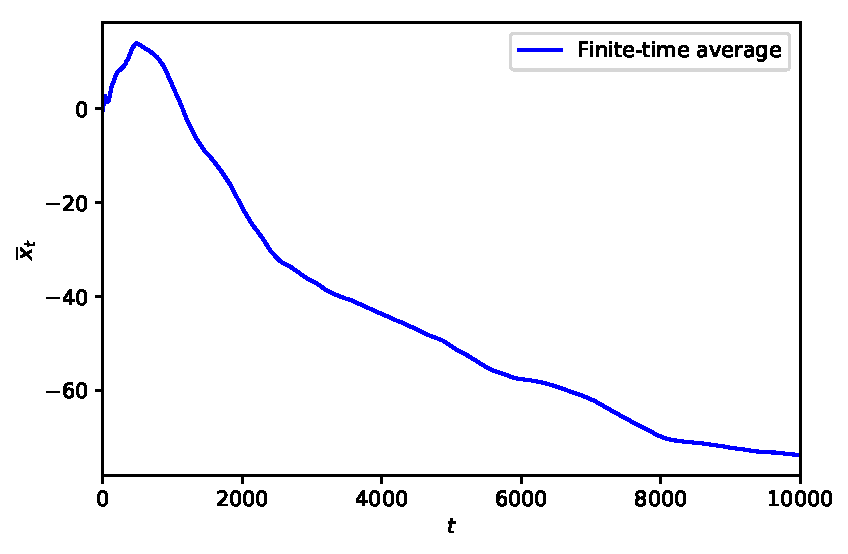
\includegraphics[width=\textwidth]{./chapter_coins/figs/BM_time_ave.pdf}}
\end{picture}
\caption{Trajectory of the finite-time average of a zero-drift \BM. The process is not ergodic: the time average 
does not converge to a number, but is instead distributed according to 
$\mN(0,\t/3)$ for all times, while the expectation value is zero. It is the result of integrating a \BM; 
integration is a smoothing operation, and as a consequence the trajectories are smoother than \BM (unlike a 
\BM trajectory, they are differentiable).}
\flabel{1_6}
\end{figure}
\FloatBarrier

\subsection{Geometric Brownian motion}
\seclabel{Geometric_Brownian}
\begin{defn}{Geometric Brownian motion}
If the logarithm of a quantity performs Brownian motion, the quantity itself performs ``geometric Brownian 
motion.''
\end{defn}

While in \secref{Brownian_motion} $\gv(\x)=\ln(\x)$ performed \BM, $\x$ 
itself performed \GBM. The change of variable from $\x$ 
to $\gv(\x)=\ln(\x)$ is trivial in a sense but it has interesting consequences. 
It implies, for instance, that 
\begin{itemize}
\item $\x(\t)$ is log-normally distributed
\item increments in $\x$ are neither stationary nor independent
\item $\x(\t)$ cannot become negative 
\item the most likely value of $\x$ (the mode) does not coincide with the 
expectation value of $\x$. 
\end{itemize}
These and other properties of the log-normal distribution will be discussed in detail in \secref{Log-normal_wealth}.
The log-normal distribution is not symmetric, unlike the Gaussian 
distribution. 

Again, it is informative to write \GBM as a stochastic differential equation. 
\be
\gd\x=\x(\gmu \gd\t+ \gsigma \gd\gW).
\elabel{GBM_c}
\ee
Trajectories for \GBM can be simulated using the discretized form
\be
\d \x=\x(\gmu \dt+ \gsigma \sqrt{\dt} \gxi_\t),
\elabel{GBM_d}
\ee
where $\gxi_\t \sim \mN(0,1)$ are instances of a standard normal variable. In such simulations
we must pay attention that the discretization does not lead to negative values of $\x$. This 
happens if the expression in brackets in \eref{GBM_d} is smaller than $-1$ (in which case $\x$ changes negatively by more than itself).
To avoid negative values we must have $\gmu \dt + \gsigma \sqrt{\dt} \gxi_\t>-1$, or 
$\gxi_\t <\frac{1+\gmu\dt}{\gsigma \sqrt{\dt}}$. As $\dt$ becomes large it becomes more likely for
$\gxi_\t$ to exceed this value, in which case the simulation fails. But $\gxi_\t$ is Gaussian distributed, meaning
it has thin tails, and choosing a sufficiently small value of $\dt$ makes these failures essentially impossible.

On logarithmic vertical scales, \GBM looks like \BM, and we've already seen some examples. 
But it is useful to look at a trajectory of \GBM on linear scales to develop an intuition for this important process.
\begin{figure}[h!]
\begin{picture}(200,230)(0,0)
    \put(0,-5){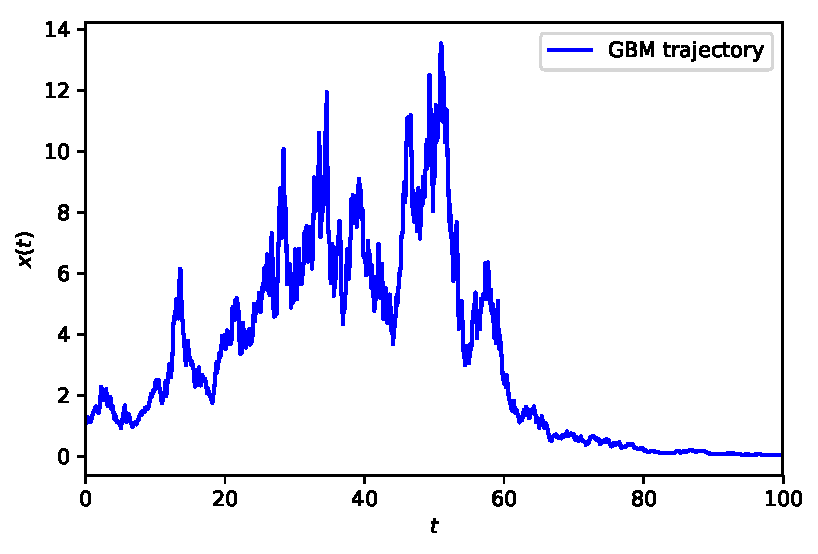
\includegraphics[width=\textwidth]{./chapter_coins/figs/GBM_trajectory.pdf}}
\end{picture}
\caption{Trajectory of a \GBM. What happens to the trajectory tomorrow depends strongly on where it is today -- for instance, unlike for \BM, it is difficult to recover
from a low value of $\x$, and trajectories are likely to get stuck near zero. Occasional excursions are characterised
by large fluctuations. Parameters are $\gmu=0.05$ per time unit and $\gsigma=\sqrt{2 \gmu}$, corresponding to zero 
growth rate in the long run. It would be easy to invent a story to go with this (completely random) trajectory --
perhaps something like  ``things were going well
in the beginning but then a massive crash occurred that destroyed morale.''}
\flabel{1_7}
\end{figure}

The basic message of the game from \secref{The_game} is that we may obtain different values for growth rates, depending on
how we average -- an expectation value is one average, a time average is quite another. The game 
itself is sometimes called the multiplicative binomial process \cite{Redner1990}, we thank \person{S. Redner} for 
pointing this out to us. \GBM is the continuous version of the multiplicative binomial process, and it shares the
basic feature of a difference between the growth rate of the expectation value and time-average growth.

The expectation value is easily computed -- the process is not ergodic, but that does not mean we cannot
compute its expectation value. We simply take the expectations values of both sides of \eref{GBM_c} to get
\bea
\ave{\gd\x}&=&\ave{\x(\gmu \gd\t+ \gsigma \gd\gW)}\\
=\gd\ave{\x}&=&\ave{\x} \gmu \gd\t.
\eea
This differential equation has the solution 
\be
\ave{\x(\t)}=\x(\tn)\exp(\gmu \t),
\ee
which determines the growth rate of the expectation value as 
\be
\gex=\gmu.
\elabel{expectation_g}
\ee

As we know, this growth rate is different from the growth rate that materializes with probability 1 in the long run. 
Computing the time-average growth rate is only slightly more complicated. 
We will follow this plan: consider the discrete process \eref{GBM_d} and compute the changes in the logarithm of $\x$, 
then we will let
$\dt$ become infinitesimal and arrive at the result for the continuous process. We know $\d \ln(\x(\t))$
to be ergodic and reflective of performance over time, wherefore we will proceed to take its expectation value to compute the time average 
of the exponential growth rate of the process. 

The change in the logarithm of $\x$ in a time interval $\dt$ is
\bea
\ln \x(\t+\dt) - \ln \x(\t) &=&\ln [\x(1+\gmu \dt+ \gsigma \sqrt{\dt} \gxi_\t)] - \ln \x(\t)\\
&=&\ln \x + \ln (1+\gmu \dt+ \gsigma \sqrt{\dt} \gxi_\t) - \ln \x(\t)\\
&=&\ln (1+\gmu \dt+ \gsigma \sqrt{\dt} \gxi_\t),
\eea
which we Taylor-expand as $\ln(1+ \text{something small})$ because we will let $\dt$ become small.
Expanding to second order,
\be
\ln \x(\t+\dt) - \ln \x(\t) =\gmu \dt+ \gsigma \sqrt{\dt} \gxi_\t - \frac{1}{2} \left(\gmu \gsigma \dt^{3/2}\gxi_\t+
\gsigma^2\dt 
\gxi_\t^2\right)+\go(\dt^2),
\ee
using ``little-o notation'' to denote terms that are of order $\dt^2$ or smaller. Finally, because
$\d \ln \x(\t)$ is ergodic, by taking the expectation value of this equation we find the
time average of $\d \ln \x(\t)$
\be
\ave{\ln \x(\t+\dt) - \ln \x(\t)} =\gmu \dt- \frac{1}{2} \left(\gmu^2\dt^2+\gsigma^2\dt \right)+o(\dt^2).
\ee
Letting $\dt$ become infinitesimal the higher-order terms in $\dt$ vanish, and we find
\be
\ave{\ln \x(\t+\gd\t) - \ln \x(\t)} =\gmu \gd\t- \frac{1}{2} \gsigma^2 \gd\t,
\ee
so that the time-average growth rate is
\be
\gt=\frac{\gd \ave{\ln \x}}{\gd\t}=\gmu - \frac{1}{2} \gsigma^2.
\elabel{time_g}
\ee

We could have guessed the result by combining Whitworth's argument on the disadvantage of
gambling with the scaling of \BM. Let's re-write the factor $1-\epsilon$ in \eref{Whitworth} as
$1-\gsigma \sqrt{\dt}$. According to the scaling of the variance in a random walk, \eref{BM_var}, 
this would be a good coarse-graining of some faster
process (with shorter time step) underlying Whitworth's game.
To find out what happens over one single time step we take the square root of \eref{Whitworth},
\be
[(1+\gsigma \sqrt{\dt})(1-\gsigma \sqrt{\dt})]^{1/2}=[1-\gsigma^2 \dt]^{1/2}.
\ee 
Letting $\dt$ become infinitesimally small, we replace $\dt$ by $\gd \t$, and the first-order
term of a Taylor-expansion becomes exact,
\be
[(1+\gsigma \sqrt{\dt})(1-\gsigma \sqrt{\dt})]^{1/2}\to 1-\frac{\gsigma^2}{2} \gd\t,
\ee 
in agreement with \eref{time_g} if the drift term $\mu=0$, as assumed by Whitworth.

\subsubsection{\Ito calculus}
\seclabel{Ito}
We have chosen to work with the discrete process here and have arrived at a result that is more
commonly shown using \Ito's formula. We will not discuss \Ito calculus in depth 
but we will use some of its results. The key insight of \Ito was that the non-differentiability
of so-called \Ito processes leads to a new form of calculus, where in particular the chain rule of
ordinary calculus is replaced.
An \Ito process is a \SDE of the following form
\be
d\x = a(\x, \t) d\t + b(\x, \t) \gd\gW.
\elabel{Ito_process}
\ee
If we are interested in the behaviour of some other quantity that is a 
function of $\x$, let's say $\gv(\x)$, then \Ito's formula tells us how to derive
the relevant \SDE as follows:
\be
d\gv =  \left(\frac{\partial \gv}{\partial\t} +a(\x, \t)\frac{\partial \gv}{\partial\x} + \frac{b(\x,\t)^2}{2} \frac{\partial^2 \gv}{\partial\x^2}\right) d\t + b(\x, \t) \frac{\partial \gv}{\partial\x} \gd\gW.
\elabel{Ito}
\ee
Derivations of this formula can be found on Wikipedia. Intuitive derivations, such as \cite{Hull2006}, use the 
scaling of the variance, \eref{BM_var}, and more formal 
derivations, along the lines of \cite{Harrison2013}, rely on integrals.
We simply accept \eref{Ito} as given. It makes it very easy to re-derive \eref{time_g}, which we leave as an exercise:
use \eref{Ito} to find the \SDE for $\ln(\x)$, take its expectation value and differentiate with respect to $\t$. 
We will use \eref{Ito} in \secref{rescaled}. The above computations are intended to 
give the reader intuitive confidence that \Ito calculus can be 
trusted\footnote{\Ito calculus is one way of interpreting the non-differentiability of \gd\gW. Another interpretation
is due to Stratonovich, which is not strictly equivalent. However, the key property of \GBM that we make
extensive use of is the difference between the growth rate of the expectation value, $\gex$, and the
time-average growth rate, $\gt$. This difference is the same in the Stratonovich and the \Ito interpretation, and all our results hold in both cases.}. 
We find that, though phrased in different words, our key insight -- that the growth rate of the expectation value is not the time-average
growth rate -- has appeared in the literature not only in 1870 but also in 1944.
And in 1956 \cite{Kelly1956}, and in 1966 \cite{Thorp1966}, and in 1991 \cite{CoverThomas1991}, and at many other times. 
Yet the depth of this insight remained unprobed.

\Eref{time_g}, which agrees with \Ito calculus, may be surprising.
Consider the case of no noise $\gd\x=\x \gmu \gd\t$. Here we can identify $\gmu=\frac{1}{\x}\frac{\gd\x}{\gd\t}$ 
as the infinitesimal increment in the logarithm, $\frac{\gd \ln(\x)}{\gd\t}$, using the chain rule of ordinary calculus. 
A na\"ive application of the chain rule to \eref{GBM_c} would therefore also yield $\frac{\gd \ave{\ln(\x)}}{\gd\x}=\gmu$, 
but the fluctuations in \GBM have a non-linear effect, and it turns out that the usual chain rule does not apply. \Ito
calculus is a modified chain rule, \eref{Ito}, which leads to the difference $-\frac{\gsigma^2}{2}$ between the 
expectation-value growth rate and the time-average
growth rate. 

This difference is sometimes called the ``spurious drift'', but at the \LML we call it the ``Weltschmerz'' because 
it is the difference between the many worlds of our dreams and fantasies, and the one cruel reality that 
the passage of time imposes on us.
